
%TODO cambiar las palabras entre []
%TODO rellenar los '...'
%TODO Hablar sobre el interprete de trazas, y la manera de leer los resultados



\documentclass[titlepage, 12pt]{book}
\usepackage[spanish]{babel}

\pagestyle{plain}
\title{Falluto2.0 Un Model Checker para la verificaci\'on autom\'atica de sistemas tolerantes a fallas.}
\author{Raul Monti}
\date{Diciembre 2012}

\usepackage{graphicx} %para poner im\'agenes
\usepackage{float}    % para establecer posici\'on de im\'agenes
\usepackage{amsmath}  % para etiquetar flechas
\usepackage{tabularx}
\usepackage{enumerate}
\usepackage{longtable}


% APENDICES
\usepackage{appendix}
\renewcommand{\appendixname}{Ap\'endices}
\renewcommand{\appendixtocname}{Ap\'endices}
\renewcommand{\appendixpagename}{Ap\'endices}
%


% Linea separadora para c\'odigo
\newcommand{\HRule}{\rule{\linewidth}{0.5mm}}
%


% MACROS

\newcommand{\X}{\mathop{\mathsf{X}}}
\newcommand{\G}{\mathop{\mathsf{G}}}
\newcommand{\F}{\mathop{\mathsf{F}}}

\newcommand{\U}{\mathbin{\textsf{U}}}
\newcommand{\R}{\mathbin{\textsf{R}}}

\newcommand{\A}{\mathbin{\textsf{A}}}
\newcommand{\E}{\mathbin{\textsf{E}}}

\newcommand{\AX}{\mathop{\mathsf{AX}}}
\newcommand{\AG}{\mathop{\mathsf{AG}}}
\newcommand{\AF}{\mathop{\mathsf{AF}}}
\newcommand{\EX}{\mathop{\mathsf{EX}}}
\newcommand{\EG}{\mathop{\mathsf{EG}}}
\newcommand{\EF}{\mathop{\mathsf{EF}}}

\newcommand{\AU}[2]{\mathsf{A}({#1}\U{#2})}
\newcommand{\EU}[2]{\mathsf{E}({#1}\U{#2})}

%

\def\Falluto20{{\rm F\kern-.1667em\lower.5ex\hbox{A}\kern-.125emllutO2.0}}

\begin{document}

%\maketitle

%%%%%%%%%%%%%%%%%%%%%%%%%%%%%%%%%%%%%%%%%%%%%%%%%%%%%%%%%%%%%%%%%%%%%%%%%%%%%%%%%%%%%%%%%%%%%%%%%%%%%%%%%%%%%%%%%%%%%%%%%%%%%%
% CARATULA
%

\begin{titlepage}
\begin{center}

% Upper part of the page. The '~' is needed because \\
% only works if a paragraph has started.

\includegraphics[width=0.30\textwidth]{./Imagenes/logo}~\\[0.5cm]

\textsc{\Large Universidad Nacional de C\'ordoba.\\ Facultad de Matem\'atica, Astronom\'ia y F\'isica}\\[0.5cm]

\textsc{\large Trabajo final de grado}\\

% Title
\HRule \\[0.4cm]
{ \huge \bfseries Falluto2.0 Un Model Checker para la verificaci\'on autom\'atica de sistemas tolerantes a fallas.}\\
\HRule \\[1.0cm]



\hspace{0.5\textwidth}
\begin{minipage}{0.45\textwidth}
\begin{flushleft}
{\large
Ra\'ul \textsc{Monti}\\
Directores:\\
Dr. Pedro R. \textsc{D'Argenio},\\
Dr. Nazareno \textsc{Aguirre}
}
\end{flushleft}
\end{minipage}

% Author and supervisor
%\begin{minipage}{0.4\textwidth}
%\begin{flushleft} \large
%\emph{Alumno:}\\
%Ra\'ul E.~\textsc{Monti}
%\end{flushleft}
%\end{minipage}
%\begin{minipage}{0.4\textwidth}
%\begin{flushright} \large
%\emph{Director:} \\
%Dr.~Pedro~R.~\textsc{D'Argenio}\\
%\emph{Codirector:} \\
%Lc.~Nazareno \textsc{Aguirre}
%\end{flushright}
%\end{minipage}

\vfill

% Bottom of the page
\begin{flushright}
{C\'ordoba, \today}
\end{flushright}

\end{center}
\end{titlepage}


%%%%%%%%%%%%%%%%%%%%%%%%%%%%%%%%%%%%%%%%%%%%%%%%%%%%%%%%%%%%%%%%%%%%%%%%%%%%%%%%%%%%%%%%%%%%%%%%%%%%%%%%%%%%%%%%%%%%%%%%%%%%%%
\newpage
~\\
%%%%%%%%%%%%%%%%%%%%%%%%%%%%%%%%%%%%%%%%%%%%%%%%%%%%%%%%%%%%%%%%%%%%%%%%%%%%%%%%%%%%%%%%%%%%%%%%%%%%%%%%%%%%%%%%%%%%%%%%%%%%%%

\newpage
\chapter*{\center{Resumen}}

Los sistemas computacionales juegan roles determinantes en muchas \'areas de nuestra vida cotidiana. En algunos casos la dependencia hacia estos sistemas es cr\'itica, y el mal funcionamiento de los mismos puede acarrear grandes perdidas econ\'omicas o hasta de vidas humanas.

Las fallas en el dise\~no del sistema, como as\'i tambi\'en aquellas fallas causadas por el entorno de ejecuci\'on, pueden llevar a un comportamiento erroneo del mismo.
%
%Los sistemas tolerantes a fallas son capaces de lidiar con la presencia de fallas y sobrellevar estas situaciones que en otros casos llevar\'ian a la aver\'ia o mal funcionamiento de los mismos. Estos sistemas por ende presentan una gran ventaja con respecto a aquellos que no lo son. Introducir la capacidad de tolerar fallas en un sistema computacional no es sencillo y es muy propenso a producir errores. La verificaci\'on de la corrección de estos sistemas es entonces de vital importancia si se busca certificar que en efecto las fallas sean toleradas.\\

Los sistemas tolerantes a fallas son capaces de lidiar con la presencia de fallas y sobrellevar estas situaciones que en otros casos llevar\'ian al mal funcionamiento de los mismos. Dar la capacidad de tolerar fallas a un sistema computacional no es sencillo y es muy propenso a introducir errores. La verificaci\'on de la corrección de estos sistemas es entonces de vital importancia.

%El model checking es una t\'ecnica formal que se encarga de verificar que el modelo de un sistema cumpla con un conjunto de propiedades. Este m\'etodo de verificaci\'on es exhaustivo y por lo tanto nos permite una verificaci\'on completa sobre el modelo del sistema a implementarse.\\

El model checking es una t\'ecnica formal que se encarga de verificar exhaustivamente que el modelo de un sistema cumpla con un conjunto de propiedades.

En este trabajo se presenta un lenguaje para el modelado de sistemas tolerantes a fallas y la especificaci\'on de propiedades sobre los mismos. Se provee adem\'as la herramienta de verificaci\'on Falluto2.0, construida como front-end para el model checker simb\'olico NuSMV, la cual utiliza el lenguaje descripto. Se analiza la simplicidad y practicidad del lenguaje como as\'i tambi\'en su corrección. Por \'ultimo se observa el uso de la herramienta sobre dos casos particulares de modelado de sistemas tolerantes a fallas.

 
\newpage
ABSTRACT
\newpage
AGRADECIMIENTOS

\newpage
\tableofcontents

\newpage


\chapter{Introducci\'on}
\label{introduccion}

Es f\'acil notar la amplia dependibilidad que las personas hemos formado alrededor de dispositivos computacionales. A medida que crece la confianza hacia estos dispositivos para la realizaci\'on de diferentes tareas, crece tambi\'en el peligro que puede acarrear la ocurrencia de una falla en los mismos. En algunos casos, las actividades a las que son dedicados estos sistemas son actividades de bajo riesgo, como por ejemplo en un reloj de pulsera o un reproductor de m\'usica, y el incorrecto funcionamiento de los mismos no ocasiona da\~nos mayores. En otros casos las actividades realizadas son de car\'acter cr\'itico, como es por ejemplo en el caso de controladores de vuelo, o controladores de compuertas de contenci\'on fluvial. Es en estos \'ultimos donde el incorrecto funcionamiento del sistema puede provocar grandes monetarias o hasta de vidas humanas.

Podemos considerar a la falla en una componente de hardware o software como una desviaci\'on de su funci\'on esperada. Las fallas pueden surgir durante todas las etapas de evoluci\'on del sistema computacional - especificaci\'on, dise\~no, desarrollo, elaboraci\'on, ensamblado, instalaci\'on- y durante toda su vida operacional \cite{faultInjection} (debido a eventos externos). Este comportamiento fuera de lo normal puede llevar a un falla funcional del sistema, provocando que se comporte de manera incorrecta, o simplemente deje de funcionar.

Es importante entonces, para lograr una mayor confiabilidad del software (confiabilidad de que se comporte como su especificaci\'on describe) tomar acci\'on sobre la ocurrencia de estas fallas. Existen diferentes enfoques para tratar con fallas. Uno de ellos es elaborar sistemas tolerantes a fallas. A diferencia de otros enfoques en los que se busca eliminar o disminuir la ocurrencia de fallas, en estos sistemas se busca disminuir los efectos de las fallas y en el mejor de los casos recuperarse de estos y evitar que acarreen en fallas funcionales del sistema.

Queda claro entonces que un sistema tolerante a fallas provee grandes ventajas en comparaci\'on a uno que no contempla la ocurrencia de las mismas. Al igual que con el resto de los sistemas computacionales, es conveniente comprobar la corrección de los sistemas tolerantes a fallas. El dise\~no de algoritmos de tiempo real distribuidos tolerantes a fallas es notoriamente dif\'icil y \emph{propenso a errores}: la combinaci\'on de la ocurrencia de fallas, conviviendo con eventos concurrentes, y las variaciones en las duraciones de tiempos reales llevan a una explosi\'on de estados que genera una gran demanda a la capacidad intelectual del dise\~nador humano \cite{SteinerRushby}.

En un mundo idealizado, los algoritmos son derivados por un proceso sistem\'atico conducido por argumentos formales que aseguran su correcci\'on respecto a la especificaci\'on original. En cambio, en la realidad contempor\'anea, los dise\~nadores suelen tener un argumento informal en mente y desarrollan el algoritmo final y sus par\'ametros explorando variaciones locales contra este argumento y contra escenarios que resalten casos dif\'iciles o problem\'aticos. La exploraci\'on contra escenarios puede ser parcialmente automatizada usando un simulador y prototipos \'agiles y esta automatizaci\'on puede llegar a incrementar el n\'umero de escenarios que ser\'an examinados y la confiabilidad de la examinaci\'on. La examinaci\'on autom\'atica de escenarios puede ser llevada a un nivel a\'un m\'as avanzado usando \emph{Model Checking} \cite{SteinerRushby}.

En ciencias de la computaci\'on \emph{Model Checking} refiere al siguiente problema: dada una estructura formal del modelo de un sistema, y dada una propiedad escrita en alguna l\'ogica espec\'ifica, verificar de manera autom\'atica y exhaustiva si el sistema satisface la propiedad. El sistema normalmente representa a un componente de hardware o software, y la f\'ormula a cumplirse representa una propiedad de \emph{safety} o \emph{liveness} que se desea verificar que el sistema cumpla, y de esta manera incrementar la confiabilidad sobre el mismo.

El reducido nivel de interacci\'on que presenta este m\'etodo con el usuario es visto como un ventaja para la aplicaci\'on en la industria, ya que incrementa las posibilidad des ser usad por individuos no expertos \cite{RuysBrinksma}. %TODO quiz\'as quitar esto y ponerlo en la seccion que sigue 
Sin embargo es preciso modelar el sistema y definir las propiedades, lidiando mientras tanto con el principal problema del Model Checking: \emph{la explosi\'on de estados} debido al incremento exponencial de los mismos a ra\'iz de la introducci\'on de variables en la especificaci\'on del sistema.

%Es objetivo de este trabajo elaborar una herramienta que logre contribuir a disminuir los problemas al momento de verificar sistemas tolerantes a fallas. Por un lado se intenta evitar la introducci\'on de errores en el modelado del sistema en el que conviven fallas con procesos concurrentes. Por otro lado se busca evitar la introducci\'on excesiva de nuevas variables al representar el comportamiento de las fallas, evitando as\'i la nociva explosi\'on de estados al momento de la verificaci\'on.

Es objetivo de este trabajo elaborar una herramienta que contribuya a disminuir el esfuerzo y a evitar la introducci\'on de errores en el modelado y verificaci\'on mediante model checking de sistemas tolerantes a fallas. Buscamos con nuestra herramienta evitar tanto la introducci\'on de errores en el modelado como as\'i tambi\'en contener la explosi\'on de estados de la cual sufre el model checking. Queremos tambi\'en que nuestro lenguaje de modelado ofrezca facilidades al momento de especificar las propiedades a verificar, de manera especial en el caso en que las mismas involucren la ocurrencia de fallas.

Para ello presentamos la herramienta de model checking \emph{Falluto2.0}, orientada a la verificaci\'on de sistemas tolerantes a fallas. Esta herramienta presenta una capa de abstracci\'on sobre NuSMV\cite{NuSMV}, un model checker basado en diagramas de decisi\'on binaria. Falluto2.0 presenta un lenguaje de car\'acter declarativo para la introducci\'on de fallas en el modelado del sistema, generando un marco de seguridad contra la introducci\'on de errores evitando que el usuario deba explicitar el funcionamiento de la falla dentro del modelo. Este trabajo se presenta como extensi\'on del trabajo realizado por Edgardo Hames\cite{Hames}, y toma como base los conocimientos adquiridos a partir del trabajo de caracter\'isticas similares realizado por Nicol\'as Bordenabe\cite{Bordenabe}.

%TODO seguir hablando del trabajo y poner la distribucion de los temas en el trabajo.





%%%%%%%%%%%%%%%%%%%%%%%%%%%%%%%%%%%%%%%%%%%%%%%%%%%%%%%%%%%%%%%%%%%%%%%%%%%%%%%%%%%%%%%%%%%%%%%%%%%%%%%%%%%%%%%%%%%%%%%%%%%%%%%%%%%%%%%%%%%%%%%%%%%%%%%%%%%%%%%%%%




\chapter{Tolerancia a fallas}

Mejorar la confiabilidad del sistema (el grado de confianza que se puede poner 
de manera justificada sobre el sistema) es usualmente presentado como el 
principal beneficio de la tolerancia a fallas. Introduciremos al comienzo de este cap\'itulo los conceptos b\'asicos de lo que entender\'emos como \textit{falla} en un sistema. Hablaremos luego de lo que significa que un sistema \textit{tolere fallas}, y concluiremos planteando el contexto en el cual nuestro trabajo tratar\'a la tolerancia a fallas.



%..................................................................................................................................................................



\section{Fallas}
Intuitivamente, y dentro del contexto que nos compete, podemos definir a una \textit{falla} (``fault'' en ingl\'es) en una componente de hardware o software como una perturbaci\'on de su estado la cual pone en peligro su correcto funcionamiento. Las fallas pueden ser introducidas en cualquier etapa de la evoluci\'on del sistema computacional en cuesti\'on -especificaci\'on, dise\~no, desarrollo, elaboraci\'on, ensamblado, e instalaci\'on- y pueden ocurrir en cualquier momento durante su vida operacional \cite{FaultInject}.

Una definici\'on ligeramente m\'as formal nos sugiere definir el termino \textit{falla} basado en la observaci\'on de que los sistemas cambian su estado como resultado de dos clases de eventos muy similares: operaciones normales de sistema y ocurrencia de fallas. Por lo tanto, un falla puede ser modelada como una no deseada (pero sin embargo posible) transici\'on de estado en un proceso \cite{Felix}.

Denotaremos con el t\'ermino \textit{error} (en ingl\'es ``failure'') al efecto no deseado que puede llegar a producir una falla en el comportamiento del sistema en cuesti\'on. Queda as\'i distinguida la falla de su posible efecto negativo sobre el comportamiento del sistema.



%..................................................................................................................................................................



\section{Sistemas tolerantes a fallas}
Existen sistemas dise\~nados para ser tolerantes a fallas: ellos o bien exhiben un comportamiento bien definido ante la ocurrencia de fallas, o bien enmascaran la falla de la componente al usuario, es decir contin\'uan proveyendo su servicio est\'andar especificado a pesar de la ocurrencia de las fallas en la componente \cite{Cristian}. Podemos entonces decir de manera vaga que la tolerancia a fallas es la habilidad que posee un sistema de comportarse de una manera bien definida ante la ocurrencia de una falla. En el momento de dise\~nar la tolerancia a fallas, un primer prerrequisito es especificar la clase de falla que ser\'a tolerada. Tradicionalmente esto se lograba usando como base alguno de los modelos de fallas est\'andares (crash, fail-stop, etc...), sin embargo puede hacerse de manera m\'as concisa especificando clases de fallas. El siguiente paso es enriquecer el sistema bajo consideraci\'on con componentes o conceptos que provean protecci\'on contra las fallas de una clase espec\'ifica \cite{FaultInject}.

En este trabajo podremos distinguir dos clases de fallas en particular. Un primer grupo de fallas es de tipo \textit{permanente}: \'estas com\'unmente representan fallas reales causadas por problemas irreversibles en la componente. Una vez que una falla permanente ocurre, permanece activa y afectando al sistema durante el resto de su ejecuci\'on. Por otro lado, un segundo grupo de fallas se caracteriza por ser de duraci\'on instant\'anea. Afectan el estado del sistema solo en los puntos espec\'ificos de se ejecuci\'on en los cuales estas fallas ocurren. Por lo tanto su efecto sobre el sistema solo resulta como consecuencia de los cambios particulares ocasionados en el momento de ocurrencia de la falla. Las mismas pueden repetirse indefinidamente durante la ejecuci\'on del sistema, permaneciendo activas solo en el momento en que afectan al sistema. Diremos que estas fallas son de clase \textit{transitoria}.

Al establecer el grado de tolerancia de fallas de un sistema, no basta solo con indicar las caracter\'isticas intr\'insecas de las fallas mismas, sino que es de inter\'es presentar el contexto de ocurrencia de estas. Por ello, al tratar con fallas, tomamos en cuenta diferentes condiciones y suposiciones sobre la ocurrencia de las mismas durante la ejecuci\'on del sistema. Muchas veces es de inter\'es por ejemplo evitar tratar situaciones en las que las fallas ocurren constantemente, ya que esto suele presentar un escenario irreal. Otras veces la ocurrencia de fallas en el modelo se observa en cantidades finitas y por lo tanto buscaremos poder establecer estos escenarios de an\'alisis tambi\'en. Todas estas condiciones nos permiten generar un contexto sobre el interleaving de las transiciones de falla y transiciones normales o buenas durante la ejecuci\'on del sistema. A partir de esto es que podemos analizar la tolerancia a fallas de manera mas espec\'ifica y certera. La tolerancia a fallas de nuestros sistemas quedar\'a entonces caracterizada no solo por el tipo de fallas sino que tambi\'en a partir de las condiciones de ocurrencia de las mismas.



%..................................................................................................................................................................



\section{Discusi\'on}
Tomando como respaldo lo analizado en este cap\'itulo, es que tomaremos una serie de decisiones sobre nuestro trabajo.

En este trabajo entonces no realizaremos mayor diferencia formal entre transiciones buenas del sistema y transiciones ocasionadas por fallas. Ambas ser\'an consideradas como transiciones posibles del sistema que podr\'an afectar o no el estado del mismo. Esto difiere del punto de vista tomado por otros trabajos como \cite[etc...]{Arora,dCTL}

Distinguiremos adem\'as como dijimos dos clases de falla, las de tipo \textit{Permanente} y las de tipo \textit{Transitorio}, y la tolerancia de los sistemas modelados con respecto a ambas clases de fallas ser\'a estudiada bajo ciertas condiciones de ocurrencia e interleaving entre estas y acciones normales.

Es importante aclarar que si bien nos ocuparemos del modelado del sistema en general y nos centraremos por momentos en la inyecci\'on de fallas sobre el mismo, no nos detendremos en temas espec\'ificos al dise\~no de la tolerancia a fallas.






%%%%%%%%%%%%%%%%%%%%%%%%%%%%%%%%%%%%%%%%%%%%%%%%%%%%%%%%%%%%%%%%%%%%%%%%%%%%%%%%%%%%%%%%%%%%%%%%%%%%%%%%%%%%%%%%%%%%%%%%%%%%%%%%%%%%%%%%%%%%%%%%%%%%%%%%%%%%%%%%%%





\chapter{Model Checking}
\label{CapMC}

En el dise\~no de software y hardware de sistemas complejos, se consume m\'as tiempo y esfuerzo en verificaci\'on que en construcci\'on. Se entiende que la aplicaci\'on de t\'ecnicas reduce y aligera los esfuerzos en verificaci\'on a la vez que acrecientan su cobertura. Los m\'etodos formales ofrecen un gran potencial para obtener una integraci\'on temprana de la verificaci\'on en el proceso de dise\~no, y para proveer de t\'ecnicas de verificaci\'on m\'as afectivas y reducir el tiempo invertido en aplicarlas \cite{prinMC}.

El \textit{Model Checking} es una t\'ecnica formal que permite la verificaci\'on exhaustiva de modelos finitos de sistemas. Logra esta verificaci\'on explorando todos los estados posibles del sistema modelado con la intenci\'on de constatar la veracidad un conjunto de propiedades sobre el mismo.

En este cap\'itulo comenzaremos revisando algunos conceptos b\'asicos para entender el funcionamiento de los \textit{model checkers} (programas utilizados para la verificaci\'on mediante model checking), y concluiremos presentando el proceso de model checking junto con algunas caracter\'isticas de este m\'etodo.





%..................................................................................................................................................................




\section{Sistemas de transiciones}
\label{LTSaK}
%TODO introducir sistemas de transicion

\subsection*{Labelled transition systems - LTS}

Llamamos \textit{sistema de transiciones etiquetadas} (en ingl\'es ``labeled transition systems'') a un tipo de maquina abstracta usada entre otras cosas para el modelado de sistemas computacionales concurrentes. Este sistema de representaci\'on est\'a compuesto por un conjunto de estados, un conjunto de etiquetas o nombres, y una relaci\'on ternaria explicando las transiciones etiquetadas desde un estado hacia otro del sistema.

Formalmente podemos decir que un LTS es una tres-upla $M = (S,S_{0},L,R)$ donde:
\begin{itemize}
\item $S$ es un conjunto de estados
\item $S_0 \subseteq S$ es un conjunto de estados iniciales
\item $L$ es un conjunto de etiquetas (nombres de transiciones)
\item $R \subseteq S \times L \times S$ es una relaci\'on ternaria de transiciones etiquetadas
\end{itemize}
Notemos entonces que si $s1$ y $s2$ son elementos en $S$, $l$ es un nombre en $L$, y $(s1,l,s2) \in R$, entonces estamos indicando que existe una transici\'on con nombre $l$ desde el estado $s1$ al estado $s2$. Usualmente, las etiquetas se utilizan para nombrar la acci\'on que la transici\'on realiza. De esta manera podemos modelar sistemas computacionales tomando cada elemento en $S$ como un estado particular del sistema y definiendo relaciones etiquetadas entre los mismos para representar su comportamiento.

En particular nos interesa para este trabajo la capacidad que otorga este formalismo para representar sincronizaci\'on entre acciones de distintas componentes del sistema. En el ejemplo de la figura \ref{figura1} encontramos dos componentes, un productor y un consumidor, ambas con su representaci\'on en t\'erminos de LTS. Podemos, a partir de ellas, definir un sistema concurrente sincronizado en el cual las transiciones de igual nombre en cada componente deben ser ejecutadas de manera sincronizada, mientras que las transiciones propias de cada componente pueden ejecutarse independientemente. Vemos el sistema resultante en la figura \ref{figura2}. En ella la transici\'on punteada y etiquetada con `Listo' representa la acci\'on sincronizada entre el productor y el consumidor. A su vez podemos ver en el estado punteado un caso de \emph{interleaving} entre los procesos sincronizados. All\'i podemos elegir entre darle paso a la acci\'on `Producir' del productor, o dejar que el consumidor realice la acci\'on `Consumir'. 

\begin{figure}[htp] %Al incluir el paquete float, [H] obliga a posicionar la imagen justo en este lugar por mas que a latex no le guste.
  \centering
    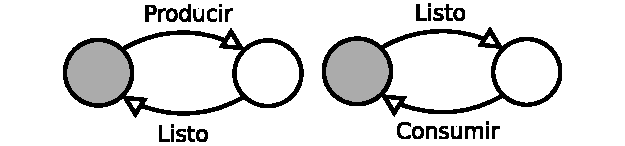
\includegraphics{Imagenes/prodYcons.pdf}
  \caption{El productor (izquierda) y el consumidor (derecha).}
  \label{figura1}
\end{figure}
~\\\\

\begin{figure}[htp] %Al incluir el paquete float, [H] obliga a posicionar la imagen justo en este lugar por mas que a latex no le guste.
  \centering
    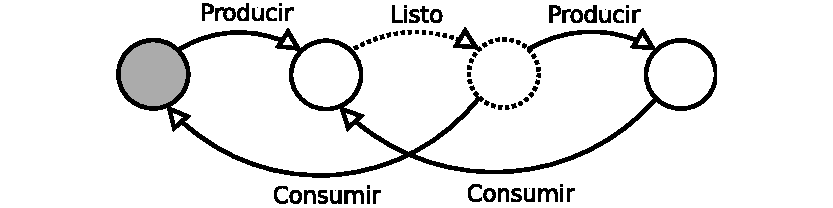
\includegraphics{Imagenes/prodYconsSincro.pdf}
  \caption{Productor y consumidor de la figura \ref{figura1} sincronizados.}
  \label{figura2}
\end{figure}


\subsection*{Estructuras de Kripke}
Una forma alternativa de describir comportamiento es a través de estructuras de Kripke. Las estructuras de Kripke son otro variante de la máquina de estados que en lugar de centrarse en la actividad observable, como hacen los LTS, se enfoca en las propiedades que satisface cada estado. Una estructura de Kripke consiste en un conjunto de estados, un conjunto de transiciones entre esos estados, y una funci\'on que etiqueta cada estado con un conjunto de propiedades que son verdaderas en este estado. Los caminos en estas estructuras modelan la ejecuci\'on del sistema \cite{Clarke}. Estas estructuras son lo suficientemente expresivas como para captar aspectos de l\'ogicas temporales tales como LTL y CTL que son lógicas mayormente usadas por los model checkers para expresar las propiedades esperadas del sistema.

Formalmente podemos definir una estructura de Kripke como sigue \cite{Clarke}:

Sea $AP$ un conjunto de proposiciones at\'omicas. Una estructura de Kripke $M$ sobre $AP$ es una cuatro-upla $(S,S_0,R,L)$ tal que:

\begin{enumerate}
\item $S$ es un conjunto finito de estados.
\item $S_0 \subseteq S$ es un conjunto de estados iniciales.
\item $R \subseteq S \times S$ es una relaci\'on de transici\'on que debe ser total, es decir, para cada estado $s \in S$ hay un estado $s' \in S$ tal que $(s,s') \in R$.
\item $L : S \rightarrow 2^{AP}$ es una funci\'on que etiqueta cada estado con el conjunto de proposiciones at\'omicas verdaderas en ese estado.
\end{enumerate}

Una ejecuci\'on del sistema desde un estado $s$ es representado en la estructura $M$ como una secuencia infinita $\pi = s_0s_1s_2...$ tal que $s_0 = s$ y $(s_i,s_{i+1})\in R$ para todo $i \geq 0$.

Notemos que podemos traducir la representaci\'on en términos de LTS de un sistema a una representaci\'on en términoes de estructuras de Kripke equivalente de la siguiente manera. Sea $M_1 = (S_1, S_{1_0} R_1, L_1)$ un sistema descripto en LTS, entonces construimos la estructura de Kripke $M_2 = (S_2,S_{2_0},R_2,L_2)$ sobre $AP$ como sigue:
\begin{itemize}
\item $ AP = \{action = e ~|~ e \in L_1 \cup \{null\}\} $
\item $ S_2 = S_1 \times (L_1 \cup \{null\}) $
\item $S_{2_0} = S_{1_0} \times \{null\}$
\item $R_2 = \{(s,a) \rightarrow (s',b) ~|~ s\overset{b}{\rightarrow}s' \in R_1, a \in L \cup \{null\}\}$
\item $L_2(s,a) = (action = a),$ para todo $(s,a) \in S_2$
\end{itemize}
Lo que hicimos fue entonces construir por cada estado $s_i$ y etiqueta $e$ en el LTS un estado en la estructura de Kripke que represente llegar al estado $s_i$ usando la etiqueta $e$. Dado que en el inicio de las ejecuciones no realizamos acci\'on alguna para llegar al estado inicial, es que hemos adem\'as definido para cada estado $s \in S_{1_0}$ un estado $(s,null)$ que lo represente en $S_2$. La funci\'on de relaci\'on se forma de manera intuitiva. El etiquetado indica qu\'e acci\'on se llev\'o a cabo para llegar a cada estado. Esto \'ultimo, junto con el nombre del estado, dejan en claro la transici\'on llevada a cabo en la ejecuci\'on del sistema definido en el LTS original. Vemos un ejemplo de traducci\'on LTS-Kripke en la figura \ref{ltsakripke}. Notemos que el sistema traducido puede ser depurado quitando estados no alcanzables como se muestra en la figura \ref{ltsakripke}.C.

\begin{figure}[htp]
  \centering
    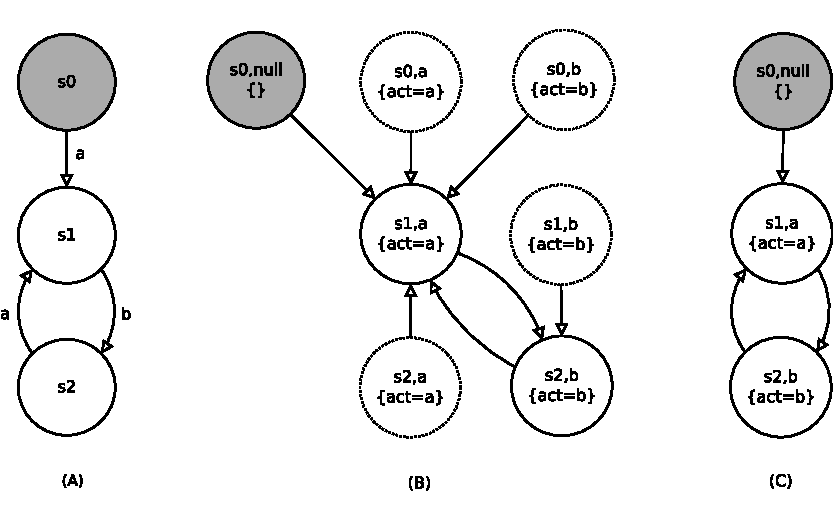
\includegraphics{Imagenes/ltsakripke.pdf}
  \caption{Ejemplo de traducci\'on de un sistema LTS a estructuras de Kripke. (A) El LTS original; (B) su traducción a estructuras de Kripke; y (C) el fragmento alcanzable de dicha estructura de Kripke}
  \label{ltsakripke}
\end{figure}




%..................................................................................................................................................................



\section{De estructuras de Kripke a f\'ormulas l\'ogicas}


Si bien las estructuras de Kripke sirven para captar intuitivamente el comportamiento de los sistemas a modelar, los model checkers trabajan sobre el modelado del sistema en base a la l\'ogica proposicional. A continuaci\'on veremos como lograr la interpretaci\'on de estructuras de Kripke usando f\'ormulas proposicionales. En lo que a nosotros concierne, la l\'ogica proposicional estar\'a comprendida por los conectivos l\'ogicos usuales - $\neg,\wedge,\vee,\rightarrow,etc...$ -, y haremos uso tambi\'en de los cuantificadores $\forall$ y $\exists$ sobre dominios finitos como generalización del $\wedge$ y del $\vee$ respectivamente.

Supongamos que queremos modelar un sistema $P$. Consideremos el conjunto de variables $V = \lbrace v_0,v_1,...,v_n \rbrace$. Consideremos para el caso que todas estas variables toman valores de un domino finito $D$. Tenemos que una valuaci\'on de $V$ es una funci\'on total sobre el dominio, la cual asigna a cada variable en $V$ un valor en $D$. Notemos que dado que los valores de las variables del sistema son las que definen el estado del mismo en su totalidad, cada valuaci\'on estar\'ia definiendo el estado del sistema. Por lo tanto un sistema P con variables V sobre el dominio D se puede representar con una estructura de Kripke $M = (S,S_0,R,L)$ sobre $AP$ donde:

\begin{itemize}
\item $AP = \{v=d~|~ v \in V, d \in D\}.$
\item Cada estado $s \in S$ es una valuaci\'on sobre $V$.
\item $R$ explica la relaci\'on entre estas valuaciones, vale decir explica la transici\'on entre los cambios de valores en las variables del sistema.
\item $L(s)$ es el subconjunto de proposiciones en $AP$ que son validas dada la valuaci\'on del estado $s$.
\end{itemize}

Dada un estado en la estructura de Kripke, es decir una valuaci\'on $s:V\rightarrow D$, podemos escribir una f\'ormula sobre las variables en $V$ tal que sea v\'alida solo para esta valuaci\'on \cite{Clarke}. La f\'ormula ser\'ia: $$(v_0 = s(v_0)) \& (v_1 = s(v_1)) \& ... \& (v_n = s(v_n))$$
Dado que en general una f\'ormula puede ser satisfecha por diferentes valuaciones, podemos a partir de ella definir el conjunto de estados que la satisfacen. As\'i por ejemplo podemos definir una f\'ormula cuyos estados que la satisfacen sean solo los estados iniciales del sistema ($S_0$ en la estructura de Kripke que lo modela).

Adem\'as de definir los estados, necesitamos poder especificar tambi\'en transiciones como f\'ormulas interpretadas de primer orden. Para ello debemos lograr a partir de una f\'ormula representar la relaci\'on entre una valuaci\'on actual y la siguiente (estado actual y estado sucesor). Necesitaremos entonces otro conjunto de variables $V'$ el cual representen las variables en estado sucesor. De esta forma, dada la f\'ormula de transici\'on $F_r$ sobre el conjunto de variables $V \cup V'$ diremos que $s'$ es estado sucesor de $s$, es decir que $(s,s')\in R$, si y solo si $F_r$ se satisface al evaluar todas sus variables en $V$ seg\'un $s$ y todas sus variables en $V'$ seg\'un $s'$.

Por \'ultimo, las proposiciones en $AP$ nos permiten definir propiedades sobre los estados. Recordemos que las proposiciones at\'omicas en $AP$ son de la forma $v=d$ con $v \in V$ y $d \in D$. Entonces tenemos que una proposici\'on $v=d$ es v\'alida en el estado $s$ si y solo si $d = s(v)$. En tal caso tenemos que $v=d \in L(s)$.




%..................................................................................................................................................................




\section{Representaci\'on de funciones booleanas en BDD}
\label{boolBDD}

Las formulas proposicionales (o funciones booleanas) son un fuerte formalismo para representar los sistemas de transiciones y razonar acerca de propiedades sobre ellos. Se busca entonces poseer una representaci\'on eficiente de estas funciones para poder abarcar sistemas considerablemente complejos. NuSMV, como as\'i tambi\'en muchos otros model checkers, logra esta representaci\'on a partir de \textit{diagramas de decisi\'on binaria (BDD)}. Los BDD presentan muchas ventajas en cuanto a eficiencia en el c\'alculo y en el espacio de almacenamiento con respecto a otras representaciones como pueden ser las tablas de verdad o subclases de la formula proposicional como la forma normal conjuntiva.

Una funci\'on booleana de $n$ argumentos es una funci\'on $f : \{0,1\}^n \to \{0,1\}$. Podemos definir a los BDD como un subconjunto de grafos dirigidos ac\'iclicos finitos con las siguientes caracter\'isticas \cite{Huth}:

\begin{itemize}
\item Poseen un \'unico nodo inicial (un \'unico nodo al cual no llega ninguna arista).
\item Todas sus hojas son etiquetadas ya sea con `0' o con `1'.
\item Todos sus nodos que no son hojas est\'an etiquetados con el nombre de una variable booleana.
\item Cada nodo (excepto las hojas) posee dos aristas salientes hacia otros nodos del diagrama, una etiquetada con `0' y otra etiquetada con `1'.
\end{itemize}

Un BDD $B$ define en sus hojas una \'unica funci\'on booleana sobre las variables en sus nodos de la siguiente manera: arrancando por el nodo inicial y dada una valuaci\'on $V=(v_1,v_2,...,v_n)$ sobre el conjunto de variables en los nodos, si $v_i$ es $0$ entonces tomo la arista saliente etiquetada con `0', de lo contrario tomo la etiquetada con `1'. Este paso se repite en cada nodo hasta llegar a un hoja. El valor de la hoja es el valor, para esa valuaci\'on, de la funci\'on booleana representada.

Podemos reducir el tama\~no de los BDD logrando una mejora de eficiencia en el espacio de memoria necesario para la representaci\'on de las funciones booleanas. Para ello usamos los siguientes tres m\'etodos \cite{Huth}:

\begin{enumerate}[R1--]
\item \textit{Remoci\'on de terminales duplicados.} Si el BDD posee m\'as de un nodo terminal `0', entonces redirigimos todas las aristas apuntando a esos nodos a uno solo de ellos y eliminamos el resto. Hacemos lo mismo con los nodos terminales `1'.
\item \textit{Remoci\'on de verificaciones innecesarias.} Si ambas aristas salientes de un nodo $n$ apuntan a un mismo nodo $m$ entonces eliminamos el nodo $n$ redirigiendo todas sus arista entrantes al nodo $m$.
\item \textit{Remoci\'on de no terminales duplicados.} Si dos nodos no terminales $n$ y $m$ son ra\'ices de sub-BDDs estructuralmente id\'enticos, entonces eliminamos uno de ellos y redirigimos todas sus aristas entrantes al otro.
\end{enumerate}

Estas reducciones no afectan la representaci\'on del BDD con respecto a la formula booleana original, y presenta una gran ventaja con respecto al espacio necesario para almacenar tablas de verdad por ejemplo. En la figura \ref{reduccionBDD} podemos ver un ejemplo de aplicaci\'on de estas reducciones. En la figura (A) vemos el BDD original. La figura (B) es el resultado de unificar las hojas seg\'un R1. La figura (C) es el resultado de eliminar uno de los nodos de etiqueta `y' según R3. Finalmente (D) es el resultado de aplicar la regla R2 eliminando el nodo de etiqueta `x'.

%TODO demasiado tonto el ejemplo?
\begin{figure}[htp]
  \centering
    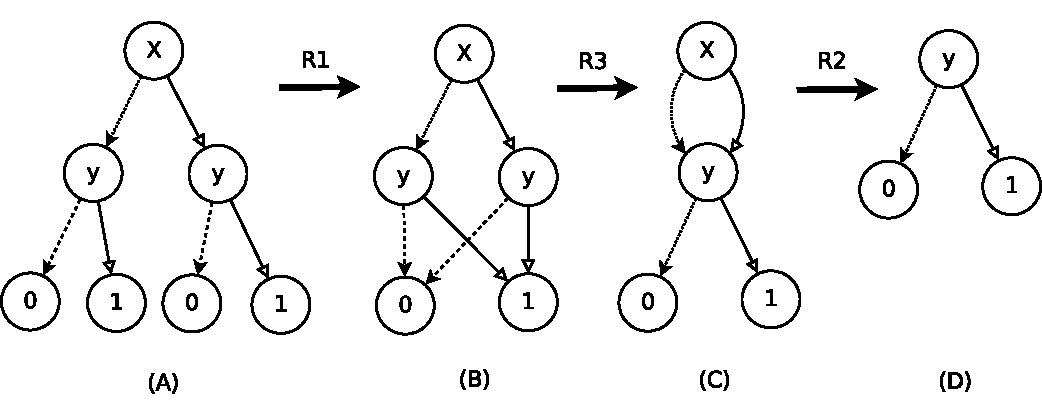
\includegraphics[scale=0.75]{Imagenes/reduccionBDD.pdf}
  \caption{Reducci\'on de un BDD seg\'un reglas R1,R2 y R3}
  \label{reduccionBDD}
\end{figure}


Si bien con estas reglas se logra reducir en gran proporci\'on cierto conjunto de BDDs, otros BDDs no son tan susceptibles a ser reducidos de esta manera. Un efecto negativo visible en mucho de estos es la reutilizaci\'on en sus nodos de una misma variable booleana, lo cual implica revisar el valor de aquellas m\'as de una vez. Otro defecto surge de que diferentes BDDs pueden representar una misma funci\'on booleana, por lo cual comparar la equidad de las funciones booleanas representadas en BDDs requiere de mucho trabajo.

Todas estas complicaciones logran ser evitadas usando un subconjunto de BDDs llamados \textit{diagramas de decisi\'on binaria ordenados} (OBDD). Los OBDD imponen un orden sobre la aparici\'on de las variables en sus nodos, evitando de este modo los BDDs con m\'as de una aparici\'on de la misma variables. Podemos dar la siguiente definici\'on de un OBDD \cite{Huth}:\\

\textit{Sea $[x_1,x_2,...,x_n]$ una lista ordenada de variables sin duplicados y sea $B$ un BDD cuyas variables pertenecen a la lista. Decimos que $B$ tiene el ordenamiento $[x_1,x_2,...,x_n]$ si todas las variables en los nodos de $B$ ocurren en la lista, y para cada ocurrencia de $x_i$ seguida de $x_j$ en cualquier camino sobre $B$, $i < j$. Decimos entonces que un OBDD es un BDD que posee un orden para alguna lista de variables.}\\

Notemos que como corolario de la definici\'on obtenemos que una variable no puede ocurrir m\'as de una vez en el OBDD. Estos diagramas poseen adem\'as la cualidad de que para cada funci\'on booleana y orden de variables existe un \'unico OBDD reducido que la representa. Osea que si $B_1$ y $B_2$ son dos OBDD reducidos con orden de variables compatible que representan a la funci\'on booleana $f$ entonces $B_1$ y $B_2$ son id\'enticos. Esto lleva a que la comparaci\'on por igualdad entre los mismos se reduzca a una simple comparaci\'on de isomorfismo. Cuando no podemos seguir reduciendo un OBDD seg\'un las reglas R1, R2 y R3, decimos que est\'a en su forma can\'onica. Son de inter\'es especial las formas can\'onicas de la figura \ref{canonicos} debido a que nos permiten identificar las siguientes situaciones:

\begin{itemize}
\item \textit{Validez de una funci\'on:} podemos verificar la validez de una funci\'on\\ booleana (verificar si la funci\'on siempre computa $1$) de la siguiente manera: reducimos su OBDD a su forma can\'onica, si el resultado de la reducci\'on es $B_1$ entonces la funci\'on es v\'alida.
\item \textit{Implicaci\'on:} podemos verificar si la funci\'on $f(x_1,x_2,...,x_n)$ implica la funci\'on $g(x_1,x_2,...,x_n)$ (es decir si $f$ computa $1$ entonces $g$ tambi\'en) reduciendo el OBDD obtenido de $f \wedge \neg g$. Si el OBDD can\'onico es $B_0$ entonces la implicación es verdadera.
\item \textit{Satisfactibilidad:} podemos verificar satisfactibilidad de una funci\'on\\ $f(x_1,x_2,...,x_n)$ (es decir si $f$ computa $1$ para alguna asignaci\'on de ceros y unos a sus variables) reduciendo su OBDD a forma can\'onica y verificando que \'esta no sea $B_0$
\end{itemize}

El orden de variables elegido toma vital importancia, ya que de \'el depende el tama\~no del OBDD. Existen algoritmos que logran un ordenamiento inteligente de las variables para mantener acotado el tama\~no de almacenamiento necesario para el OBDD. As\'i tambi\'en existen algoritmos que hacen eficiente la reducci\'on de OBDDs a su OBDD can\'onico, como tambi\'en algoritmos que permiten computar conjunci\'on, disyunci\'on y negaci\'on de OBDDs con considerable eficiencia.


\begin{figure}[htp]
  \centering
    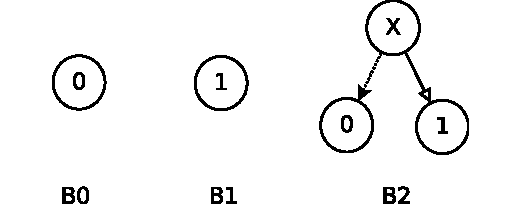
\includegraphics[scale=0.5]{Imagenes/canonicos.pdf}
  \caption{OBDDs can\'onicos de relevancia}
  \label{canonicos}
\end{figure}



El uso de BDDs produjo un gran salto en el model checking llevando en principios de los noventa a lograr verificar sistemas con espacios de estados mucho m\'as grandes que con m\'etodos anteriores. El model checking usando OBDDs es llamado \textit{Model Checking Simb\'olico} y debe su nombre a que sugiere no representar cada estado por separado, sino que los OBDDs representan los conjuntos de estados de manera simb\'olica. Veremos ahora como representar estos conjuntos de estados en OBDDs y como representar la relaci\'on de transici\'on entre ellos.

Recordemos que en nuestro modelo de sistema como estructura de Kripke hab\'iamos definido un conjunto de proposiciones at\'omicas sobre las variables del sistema, que represent\'abamos a cada estado como una valuaci\'on sobre las variables del sistema, y que la funci\'on de etiquetado $L$ nos proporcionaba el subconjunto de $AP$ que era v\'alido en cada estado. Supondremos que hay un orden sobre las proposiciones en $AP$ dado como $(x_1,x_2,...,x_n)$ donde cada $x_i$ representa una proposición atómica y representaremos cada estado $s$ como un vector $(v_1,v_2,...,v_3)$ donde $v_i \in \lbrace 0,1 \rbrace$ y $v_i = 1$ si y solo si $x_i \in L(s)$. Vemos entonces que los estados son representados por la funci\'on caracter\'istica inducida por $L$. Es decir, la funci\'on booleana que representa un estado es aquella que valuada en $(v_1,v_2,...,v_3)$ computa el valor $1$, y para cualquier otro valuaci\'on de sus variables computa el valor $0$. En t\'erminos de OBDDs, el OBDD que representa al estado $s$ es aquel que codifica la funci\'on booleana : $$l_1 \wedge l_2 \wedge ... \wedge l_n$$ donde $l_i$ es $x_i$ si $x_i \in L(s)$ y $\neg x_i$ de lo contrario. Luego para un conjunto de estados $S = {s_1, s_2, ..., s_m}$ la representaci\'on en OBDD esta dada por aquel que codifica a la funci\'on booleana $$(l_{11} \wedge l_{12} \wedge ... \wedge l_{1n}) \vee (l_{21} \wedge l_{22} \wedge ... \wedge l_{2n}) \vee ... \vee (l_{m1} \wedge l_{m2} \wedge ... \wedge l_{mn})$$ donde $(l_{i1} \wedge l_{i2} \wedge ... \wedge l_{in})$ representa al estado $s_i$.\\

Para el caso de la relaci\'on de transici\'on recordemos que \'esta es un subconjunto sobre $S\times S$. De nuevo podemos inducir la funci\'on booleana representante a partir de la funci\'on de etiquetado $L$. De este modo una relaci\'on $s\rightarrow s'$ en $R$ es representada por los vectores $(v_1,v_2,...,v_n),(v'_1,v'_2,...,v'_n)$, donde $v_i = 1$ si $p_i \in L(s)$ y $0$ en caso contrario, y $v'_i = 1$ si $p_i \in L(s')$ y $0$ en caso contrario. Una transición queda representada por el OBDD de la funci\'on booleana $$(l_1,l_2,...,l_n) \wedge (l'_1,l'_2,...,l'_n)$$ y el conjunto representando el total de la relaci\'on $R$ se logra a partir de la conjunci\'on de cada una de estas f\'ormulas.








%TODO ver qu\'e hizo Pablo Dal Lago con esto, para ampliar la teor\'ia de reducci\'on.

%..................................................................................................................................................................





\section{L\'ogicas temporales}
Las l\'ogicas temporales son lógicas modales que permiten describir y razonar sobre proposiciones en t\'erminos del tiempo. En el caso del model checking, son de gran utilidad para la especificaci\'on de las propiedades a verificar sobre el modelo del sistema. A continuaci\'on presentaremos dos l\'ogicas temporales de inter\'es para este trabajo. Ambas l\'ogicas difieren en expresividad, por lo que hacer uso de las dos nos permite una mayor versatilidad al momento de especificar las propiedades deseadas.

\subsection*{LTL}
La \textit{L\'ogica de Tiempo Lineal (LTL)} permite razonar sobre ejecuciones lineales a trav\'es del tiempo. Estas ejecuciones solo permiten ver los cambios de estado que se producen a lo largo del tiempo y cómo estos se ordenan temporalmente, pero no permiten ver el transcurso preciso del tiempo. As\'i, cada momento vvisible representa una configuraci\'on en el estado del sistema y cada salto en el tiempo representa una transici\'on desde un estado del sistema a uno nuevo. Estas l\'ogicas est\'an compuestas por un conjunto finito de proposiciones at\'omicas $AP$, los conectivos booleanos $\neg$, $\wedge$, $\vee$, $\rightarrow$, $\leftrightarrow$ y los conectivos temporales $G, F, X, U, R$. Estos \'ultimos conectivos se corresponden con las palabras en idioma ingl\'es $G$lobally, $F$inally, ne$X$t, $U$ntil y $R$elease. A continuaci\'on damos una descripci\'on intuitiva del significado de cada conectivo:

\begin{itemize}
\item $\G \phi$ expresa que en todo momento durante la ejecución se satisface la fórmula $\phi$.
\item $\F \phi$ expresa que en algún momento en el futuro se satisface la fórmula $\phi$.
\item $\X \phi$ expresa que $\phi$ se satisface en el momento inmediatamente posterior al actual.
\item $\phi \U \psi$ expresa que $\psi$ se satisface en alg\'un momento, y para todo momento anterior a aquel $\phi$ se satisface.
\item $\phi \R \psi$ expresa que o bien $\phi$ no se satisface nunca y $\psi$ se satisface siempre, o bien $\psi$ se satisface en cada momento hasta que $\phi$ se satisfaga.
\end{itemize}

Usando LTL podemos expresar propiedades de \textit{liveness} y \textit{safety} de nuestro sistema de manera sencilla. Por ejemplo para expresar \textit{``En alg\'un momento algo bueno suceder\'a''} usamos  $F$ ``algo bueno'', o para expresar \textit{``En ning\'un momento algo malo sucede''} usar\'iamos $G$ $\neg$ ``algo malo''.

Las fórmulas LTL se interpretan usualmente sobre ejecuciones de estructuras de Kripke, y si queremos saber si la formula $\phi$ se satisface en un sistema representado por la estructura de Kripke $M$, basta con ver que el lenguaje de $M$ (i.e. todas las ejecuciones posibles en $M$) satisfaga $\phi$. Definimos la sem\'antica de formulas LTL como sigue:

Sea la palabra $\omega$ = $s_1s_2s_3...$ de valuaciones en $AP$. Definimos la relaci\'on de satisfactibilidad $\models$ de una formula LTL con respecto a la palabra $\omega$ a partir de las siguientes reglas:
\begin{itemize}
\item $\omega \models p $ si $ p \in L(\omega[0])$
\item $\omega \models \neg p $ si no $\omega \models p$
\item $\omega \models \phi \vee \psi$ si $\omega \models \phi$ o $\omega \models \psi$
\item $\omega \models \X \phi$ si $\omega[1...] \models \phi$
\item $\omega \models \phi \U \psi$ si existe $i \geq 0$ tal que  $\omega[i...] \models \psi$ y para todo $0 \leq k < i$, $\omega[k...] \models \phi$ 
\end{itemize}
donde $\omega[i...]$ es el i-ésimo sufijo de $\omega$.

Notar que los dem\'as conectivos son derivados de aquellos para los que hemos definido las reglas de satisfactibilidad: $F \phi \equiv true U \phi, G \phi \equiv \neg F \neg \phi$ y $\phi R \psi \equiv \neg(\neg\phi U \neg\psi).$

Muchas veces es de inter\'es en model checking definir propiedades bajo \textit{condiciones de equidad (en ingl\'es ``Fairness Conditions'')} . Por ejemplo en el contexto del modelado de un planificador de tareas podemos requerir que el mismo atienda equitativamente a los diferentes procesos. LTL, a diferencia de CTL, nos da la posibilidad de definir estas equidades:

\begin{enumerate}
\item Equidad incondicional:\\[0.3cm] $\G~\F~p$ (a menudo se cumple $p$)
\item Equidad fuerte:\\[0.3cm] $\G~\F~q \rightarrow \G~\F~p$ (si $q$ se satisface a menudo, entonces $p$ también)
\item Equidad d\'ebil:\\[0.3cm] $\F~\G~q \rightarrow \G~\F~p$ (si en algún momento $q$ se satisface como invariante, entonces $p$ debe satisfacerse a menudo)
\end{enumerate}

En 2 y en 3, $q$ podría verse como la condición de habilitación de $p$.

\subsection*{CTL}
A diferencia de LTL, la \textit{L\'ogica de \'arbol computacional (en ingl\'es ``Computation tree logic'' (CTL))} considero toda posible bifurcación de la ejecución. Por lo tanto, una fórmula CTL puede hacer referencia a cualquier ejecución que se desprenda de cualquier estado considerado. Adem\'as de los conectivos l\'ogicos y temporales introducidos en LTL, CTL implementa el uso de los cuantificadores $\A$ (para todo camino) y $\E$ (existe un camino). De hecho, CTL requiere que todo operador temporal esté cuantificado. Esto hace que las fórmulas sean interpretadas en estados en lugar de caminos y las cuantificaciones hacen referencia a la existencia o universalidad de los caminos partiendo de un estado. As\'i es que podemos especificar propiedades como  $\EX~p$ y $\AG~\EF~p$, las cuales no pueden ser especificadas en LTL ya que en ella no podemos hablar de la existencia de al menos un camino en el futuro en el cual se cumple $p$.

Los conectivos ${\neg,\wedge,\AX,\EX,\E\U}$ comprenden un conjunto completo de conectivos para la l\'ogica CTL dado que los dem\'as pueden ser derivados a partir de ellos. Podemos decir que el siguiente es el significado intuitivo de estos conectivos:

\begin{itemize}
\item $\neg$ es la negaci\'on booleana usual.
\item $\wedge$ es la conjunci\'on booleana usual.
\item $\AX~\phi$ se cumple en un estado $s$ si para cualquier ejecuci\'on, $\phi$ se satisface en todo estado sucesor de $s$.
\item $\EX~\phi $ se cumple en un estado $s$ si existe al menos una ejecuci\'on con un estado sucesor a $s$ y donde $\phi$ se satisface.
\item $\E[\phi~\U~\psi]$ se cumple en un estado $s$ si existe al menos una ejecuci\'on $s_1s_2...s_n...$ con $s_1 = s$ con un estado $s_k$ donde $\psi$ se hace verdadero y $\phi$ se satisface en cada estado $s_i, 1 \leq i \leq n-1$.
\end{itemize}

A continuaci\'on, utilizando estructuras de Kripke, definimos la sem\'antica formal de CTL por inducci\'on estructural sobre una f\'ormula $\phi$. Sea la estructura de Kripke $M =(S,S_0,R,L)$ sobre $AP$, sea $\phi$ una f\'ormula CTL bien formada sobre $AP$, y sean $s \in S$ y $p \in AP$:\\


% TODO arreglar esta tabla para que no quede fuera del margen derecho
\begin{tabularx}{\textwidth}{@{\textbullet}lcX}
$~M,s \models p$ & $\leftrightarrow$ & $p \in L(s)$\\
$~M,s \models \neg\phi $ & $\leftrightarrow$ & $M,s \not\models \phi$\\
$~M,s \models \phi_0 \wedge \phi_1 $ & $\leftrightarrow$ & $ M,s \models \phi_0 \text{ y } M,s \models \phi_1$\\
$~M,s \models \AX\phi $ & $\leftrightarrow$ & $ \forall (s,s') \in R,~ M,s' \models \phi$\\
$~M,s \models \EX\phi $ & $\leftrightarrow$ & $ \exists (s,s') \in R$, tal que $M,s' \models \phi$\\
$~M,s \models \E(\phi_0 \U \phi_1) $ & $\leftrightarrow$ & $\exists$ una ejecuci\'on $\omega$ definida por $R$ tal que $\omega[0] = s$ y $\exists n \geq 0 ~M,\omega[n] \models \phi_1,$ y $\forall 0<i<n~ M, \omega[i] \models \phi_0$\\
\end{tabularx}




%..................................................................................................................................................................




\section{Caracter\'isticas del Model Checking}

Existen diferentes m\'etodos para la verificaci\'on de sistemas complejos, entre ellos podemos destacar como principales la simulaci\'on, el testing, la verificaci\'on deductiva, y el model checking \cite{Clarke}. Tanto la simulaci\'on como el testing comprenden realizar experimentos antes de desplegar el sistema en el campo. Mientras que en el caso de la \textit{simulaci\'on} se trabaja sobre una abstracci\'on o modelo del sistema, en el \textit{testing} se trabaja sobre el producto real. En cuanto a costo-eficiencia, estos m\'etodos pueden ser ventajosos para detectar gran cantidad de errores. Sin embargo, revisar todas las posibles interacciones y potenciales errores usando simulaci\'on y testing es prácticamente imposible.

El t\'ermino \textit{verificaci\'on deductiva} normalmente refiere al uso de axiomas y reglas para probar la corrección del sistema. Este m\'etodo si bien posee la ventaja de poder probar corrección sobre sistemas de estados infinitos no es muy utilizado fuera de casos cr\'iticos. Esto se debe a que requiere de gran cantidad de tiempo y de la conducci\'on por parte de expertos en el campo del razonamiento l\'ogico.

El \textit{Model checking} es un m\'etodo autom\'atico para la verificaci\'on de propiedades sobres sistemas concurrentes finitos. Trabaja sobre un modelo del sistema y explora exhaustivamente todos sus posibles estados con el fin de verificar si una propiedad especificada sobre el mismo es verdadera o no. Presenta ciertas ventajas sobre los m\'etodos anteriormente mencionados:

\begin{itemize}
\item Detecta errores en etapas tempranas de dise\~no, evitando tener que replantear todo al encontrar estos errores en etapas posteriores.

\item Gran parte de su proceso es autom\'atico, por lo cual no requiere de personal experto en campos de la matem\'atica para llevar a cabo las tareas de verificaci\'on.

\item Es exhaustivo con respecto al conjunto de estados del sistema.

\item Ofrece clara evidencia del problema en el caso de encontrar que la propiedad deseada sobre el sistema no se cumpla.
\end{itemize}

Sin embargo el \textit{model checking} sufre del problema de la explosi\'on de estados. Esto implica que f\'acilmente se llegue a sistemas en los que la cantidad de estados es tan grande que supera los l\'imites de memoria f\'isica del hardware sobre el que corre el programa de model checking. Muchos algoritmos y optimizaciones sobre los model checkers han ayudado a combatir este efecto, pero sin embargo el mismo persiste. Otra soluci\'on a este problema es llevar el modelado a una mayor abstracci\'on con el fin de disminuir la cantidad de estados finales. Al hacer esto debemos tomar en cuenta que la abstracci\'on debe asegurar que las propiedades que no se satisfacen en el sistema concreto, tampoco se satisfagan en el modelo abstracto.

Christel Baier y Joost-Pieter Katoen \cite{Baier} identifican las siguientes tareas como pasos para realizar el \textit{proceso de model checking} sobre el dise\~no de un sistema (ver también la figura \ref{procMC}):

\begin{enumerate}
\item Fase de modelado:
\begin{itemize}
\item Modelar el sistema en consideraci\'on usando el lenguaje del model checker que se tenga a mano.
\item Realizar algunas simulaciones sobre el modelo como primera revisi\'on y r\'apida aceptaci\'on del mismo.
\item Describir las propiedades a verificar sobre el modelo usando el lenguaje espec\'ifico para esta tarea.
\end{itemize}
\item Fase de ejecuci\'on:\\\\
Ejecutar el model cheker para verificar la validez de una propiedad sobre el sistema modelado. 
\item Fase de an\'alisis:
\begin{itemize}
\item Si la propiedad result\'o ser v\'alida $\longrightarrow$ en el caso de haber m\'as propiedades a verificar, proceder con la verificaci\'on de las mismas.
\item Si la pripiedad fu\'e refutada $\longrightarrow$
\begin{enumerate}
\item analizar, a partir de simulaci\'on, el contraejemplo generado.
\item refinar el modelo, dise\~no o propiedad.
\item repetir todo el proceso.
\end{enumerate}
\item La computadora se qued\'o sin memoria $\longrightarrow$ intentar reducir el modelo y empezar de nuevo.
\end{itemize}
\end{enumerate}


\begin{figure}[htp]
  \centering
    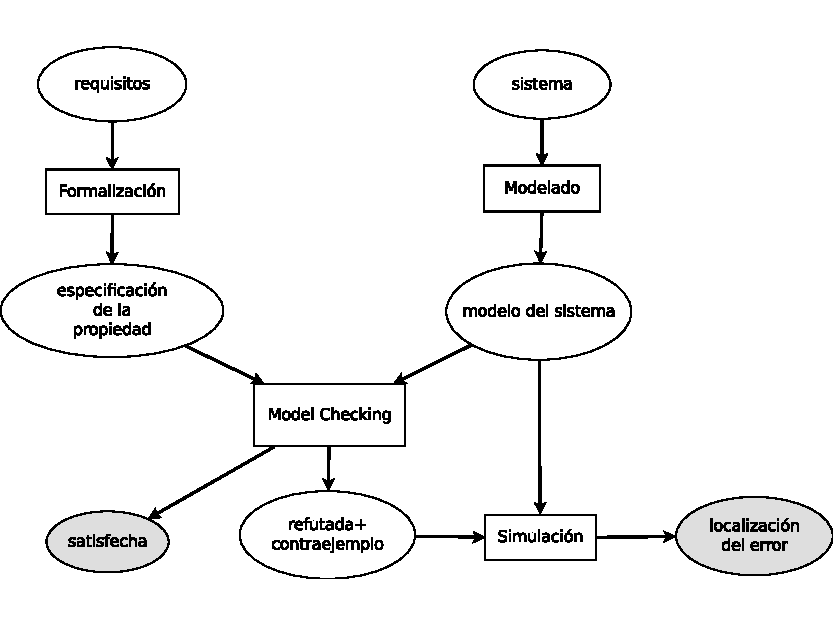
\includegraphics{Imagenes/procesoMC4.pdf}
  \caption{El proceso de Model Checking}
  \label{procMC}
\end{figure}


En la fase de modelado podemos distinguir entonces por un lado el modelado del sistema y por otro la especificaci\'on de las propiedades. El modelado del sistema, si bien algunas veces suele ser una simple compilaci\'on al lenguaje de modelado espec\'ifico de la herramienta de model checking, otras veces puede requerir depuraci\'on del modelo para eliminar caracter\'isticas innecesarias que puedan ocasionar una explosi\'on de estados a tal grado de agotarse la memoria. Por otro lado podemos destacar como asunto importante en la etapa de especificaci\'on de propiedades el hecho de lograr completitud sobre las caracter\'isticas deseadas del sistema. Es decir que es esencial en esta etapa lograr expresar en las propiedades el conjunto completo de caracter\'isticas que se desea que el sistema posea.

La fase de ejecuci\'on usualmente es autom\'atica y solo consta de proveer al model checker con el modelado del sistema y la especificaci\'on de una propiedad para que el mismo decida sobre su validez.

Por \'ultimo, es en la fase de an\'alisis donde podemos decidir ya sobre el resultado de la verificaci\'on. Se pueden presentar varios escenarios: por un lado puede que el proceso de verificaci\'on no se haya completado debido al agotamiento de memoria, en cuyo caso se deber\'a recurrir al refinamiento del sistema para conseguir disminuir la explosi\'on de estados%, o bien se deber\'a usar un equipo de mayor potencial en el caso de que ya no se logre llegar a un refinamiento significativo. 
Puede ser el caso de que todas las propiedades hayan sido validadas por el model checker, lo que indicar\'ia que el modelo del sistema cumple con las caracter\'isticas expresadas en la especificaci\'on de las propiedades. Por \'ultimo puede suceder que una o m\'as propiedades hayan sido refutadas. En este caso, la herramienta provee un contraejemplo que nos permite identificar el problema, el cual puede haber sido causado por una mal modelado del sistema, una falla en la especificaci\'on, o simplemente porque en efecto el sistema no cumple con la caracter\'istica deseada.\\

Es importante tomar en cuenta que el \'exito de la verificaci\'on depende fuertemente de la corrección en el modelado del sistema y la especificaci\'on de las propiedades. El sistema puede tener errores pero haber sido modelado evitando los mismos, lo cual puede llevar a que el model checker entregue falsos positivos. Este efecto tambi\'en puede ser causa de una especificaci\'on incompleta o err\'onea de las caracter\'isticas a verificar.\\

\section{Discusi\'on}
Veremos m\'as adelante, al momento de presentar las sintaxis de NuSMV y Falluto2.0, como se pone en pr\'actica la teor\'ia presentada en este cap\'itulo. Podremos distinguir por un lado que el lenguaje presentado por Falluto2.0 para modelar los sistemas se acerca en gran medida a la idea de LTS, mientras que por otro lado el de NuSMV ser\'a m\'as cercano a la representaci\'on de estructuras de Kripke. Esto nos llevar\'a a que la teor\'ia de traducci\'on de LTS a f\'ormulas de Kripke presentada en la secci\'on \ref{LTSaK} conforme la base de la sem\'antica de compilaci\'on de Falluto2.0.\\
 
Este cap\'itulo nos deja entrever as\'i tambi\'en el gran control que tendremos sobre el sistema final que el model checker verificar\'a, dado que al describir la estructura de Kripke estamos a un paso del armado de los BDD sobres los cuales la herramienta verificar\'a el modelo. La ausencia de pasos intermedios evita la introducci\'on de nuevas variables y la complejizaci\'on del modelo la cual se traduce en una explosi\'on de estados.




%%%%%%%%%%%%%%%%%%%%%%%%%%%%%%%%%%%%%%%%%%%%%%%%%%%%%%%%%%%%%%%%%%%%%%%%%%%%%%%%%%%%%%%%%%%%%%%%%%%%%%%%%%%%%%%%%%%%%%%%%%%%%%%%%%%%%%%%%%%%%%%%%%%%%%%%%%%%%%%%%%



\chapter{NuSMV}
\section{El model checker NuSMV}

NuSMV es un model checker simb\'olico originado en la reingenier\'ia, reimplementaci\'on y extensi\'on de SMV, el primer model checker basado en BDD. NuSMV fue dise\~nado para ser una plataforma bien estructurada, de c\'odigo abierto, flexible, y ampliamente documentada, para el model checking. Con el fin de permitir que NuSMV sea utilizado en proyectos para la transferencia de tecnolog\'ias, fue dise\~nado para ser muy robusto, cercano a los est\'andares industriales, y para permitir lenguajes de especificaci\'on ampliamente expresivos \cite{Cimatti}.

NuSMV permite la verificaci\'on de propiedades en los formalismos LTL y CTL, sobre modelados finitos de sistemas concurrentes, bajo condiciones de fairness.

Para este trabajo usamos como back-end el model checker \textit{NuSMV2} \cite{NuSMV2}, el cual integra la verificaci\'on en base a \textit{BDD} junto con la verificaci\'on acotada de propiedades LTL mediante \textit{SAT-Solving}. Otra particularidad de esta versi\'on es el uso de una licencia \textit{OpenSource} para programaci\'on y distribuci\'on abierta de su c\'odigo, lo cual permite, a cualquier persona interesada, usar la herramienta gratuitamente y colaborar con el desarrollo de la misma.


\section{Lenguaje de modelado de NuSMV}
Si bien el lenguaje de modelado de NuSMV es amplio y ofrece diferentes posibilidades para la definici\'on de la maquina de estados, presentaremos en esta secci\'on solo aquella porci\'on que nos servir\'a m\'as adelante para compilar los modelos descriptos en el lenguaje de Falluto2.0.

Cada proceso del sistema se describe en NuSMV como un m\'odulo, introducido por la palabra \texttt{MODULE}. Al menos uno de estos m\'odulos debe llamarse \textit{main}, y ser\'a el m\'odulo evaluado por el interprete. Podemos ver cada proceso como una maquina de estados independiente y al conjunto de estos y sus interacciones como la maquina de estados que representa al sistema completo. Veamos entonces como definir la maquina de estado de cada proceso:

\subsection*{Variables}

Dentro de cada \textit{m\'odulo}, introduciendo la secci\'on de variables por la palabra \texttt{VAR}, definimos las variables del proceso junto con sus dominios. Poseemos tres tipos b\'asicos de variables, las booleanas, las enteras y las enumeradas. Tenemos la posibilidad de declarar una variable como un arreglo de valores de cualquiera de los tipos anteriormente mencionados. Vemos un ejemplo a continuaci\'on:
\begin{verbatim}
MODULE main
    VAR
        var1 : boolean;
        var2 : -2..3;
        var3 : {a1, something, 42};
        var4 : array -1..2 of boolean;
\end{verbatim}
Vemos que en el ejemplo la variable \texttt{var1} es de tipo booleano (su dominio est\'a formado por los valores \texttt{TRUE} y \texttt{FALSE}) , \texttt{var2} es de tipo entero y su dominio se extiende desde el numero -2 al 3 y \texttt{var3} es de tipo enumerado y su dominio lo forman las 3 palabras encerradas en llaves. Por \'ultimo \texttt{var4} es un vector de cuatro booleanos indexado sobre el rango -1 .. 2. Notemos que las valuaciones sobre las variables representan el estado del proceso y una valuaci\'on sobre el conjunto de todas las variables de cada proceso representa el estado del sistema completo, tal como se remarcó en la teoría presentada en el capítulo \ref{CapMC}.

\subsection*{Estado inicial}

Para definir el conjunto de estados iniciales de cada proceso introducimos una nueva secci\'on dentro del m\'odulo usando la palabra clave \texttt{INIT}, y hacemos uso de una f\'ormula proposicional sobre las variables del m\'odulo para restringir el subconjunto de estados que deseamos sea el inicial. Recordemos que seg\'un lo visto en la secci\'on \ref{boolBDD} para cualquier conjunto de estados podemos definir una f\'ormula tal que solo ellos la cumplan.
\begin{verbatim}
MODULE auto
    VAR
        estado: {encendido, apagado}
        nafta: 0..3
    INIT
        estado = apagado & nafta = 3
\end{verbatim}


\subsection*{Transiciones}

La palabra clave \texttt{TRANS} en NuSMV permite introducir dentro de los m\'odulos una secci\'on donde definir las transiciones de nuestra maquina de estados. As\'i como ya hemos planteado anteriormente, las transiciones hablar\'an sobre dos clases de estados: los estados actuales, y los estados posteriores, de manera de definir la relaci\'on sobre los mismos. Dada una variable de estado \texttt{x}, tenemos que \texttt{next(x)} representa el estado de la variables en el momento inmediatamente posterior al actual. Una formula proposicional establece entonces las caracter\'isticas de la relaci\'on de transici\'on. Las ambigüedades en esta f\'ormula con respecto a la maquina de estados representada introducen una elecci\'on aleatoria por parte de NuSMV. Esto es \'util para representar no determinismo entre saltos de estados.

\begin{verbatim}
MODULE auto
    VAR
        estado: {encendido, apagado}
        nafta: 0..3
    INIT
        estado = apagado & nafta = 3
    TRANS
        ( estado = encendido & nafta <= 0 ) 
        -> 
        ( next(estado) = apagado )

\end{verbatim}

Notemos que en el ejemplo solo definimos condiciones para el caso en que \texttt{estado = encendido} y \texttt{nafta <= 0}, caso en el que el auto deber\'ia apagarse en el pr\'oximo estado. En los casos en que se da \texttt{estado = apagado} o \texttt{nafta > 0} el no-determinismo maneja la elecci\'on de un estado posterior.


\subsection*{Restricciones y fairness}

NuSMV permite establecer restricciones de fairness sobre la ejecuci\'on de nuestro sistema. Esto permite revisar nuestro sistema bajo ciertos supuestos con respecto a su ejecuci\'on. Tenemos la posibilidad de definir dos tipos de condiciones de fairness sobre nuestro sistema modelado:
\begin{itemize}

\item \textit{Fairness incondicional} Dada una f\'ormula $q$ sobre el estado del sistema, escribimos \texttt{FAIRNESS q} para establecer una la condici\'on de fairness incondicional sobre nuestro sistema modelado. Establece que cierta condici\'on $q$ se cumple frecuentemente durante la ejecuci\'on del sistema. En t\'erminos de l\'ogicas de tiempo lineal, esto corresponder\'ia a restringir la ejecuci\'on del sistema a solo aquellas trazas donde se cumpla $\G \F q$.

\item \textit{Strong Fairness} Dadas dos f\'ormulas $p$ y $q$ sobre el estado del sistema, escribimos \texttt{COMPASSION(p,q)} para establecer una condici\'on de fairness fuerte sobre el sistema. Esta condici\'on restringe a la revisi\'on de aquellas ejecuciones del sistema en donde valga que si $p$ se cumple siempre a menudo entonces $q$ se cumple siempre a menudo. En t\'erminos de LTL esto corresponder\'ia a revisar solo aquellas ejecuciones donde se cumpla $\G \F p \rightarrow \G \F q$.

\end{itemize}

\subsection*{Propiedades y verificaci\'on}

NuSMV permite verificar tanto propiedades LTL como CTL sobre nuestro sistema. Para cada una de ellas tenemos su respectiva palabra clave y la precedemos con la f\'ormula que exprese la propiedad a verificar. La verificaci\'on de estas propiedades se realizara bajo las condiciones que establecen las restricciones de fairness definidas. A continuaci\'on mostramos un ejemplo que ilustra la especificaci\'on de las propiedades:

\begin{verbatim}
MODULE auto
    VAR
        estado: {encendido, apagado}
        nafta: 0..3
    INIT
        estado = apagado & nafta = 3
    TRANS
        ( estado = encendido & nafta <= 0 ) 
        -> 
        ( next(estado) = apagado )

FAIRNESS nafta > 0

LTLSPEC F nafta = 0
CTLSPEC EG estado = apagado
\end{verbatim}

En el ejemplo de arriba podemos encontrar la especificaci\'on de una propiedad LTL introducida por la palabra clave \texttt{LTLSPEC} y una CTL introducida por la palabra clave \texttt{CTLSPEC}. Ambas ser\'an verificadas sobre el sistema modelado pero bajo la condici\'on de fairness dada por \texttt{FAIRNESS F nafta = 0}.

\section*{Discusi\'on}

Si bien el lenguaje de NuSMV presenta una amplia variedad de posibilidades para el modelado del sistema, nosotros solo haremos caso a una peque\~na parte de este. Con la porci\'on del lenguaje presentado en este cap\'itulo ser\'a suficiente para describir la maquina de estados de nuestros modelos compilados de manera completa. Nos permitir\'a adem\'as mantener un claro control sobre el tama\~no de nuestro sistema al momento de compilar lo modelado por el usuario en el lenguaje de front-end que presenta Falluto2.0 al lenguaje del back-end ofrecido por NuSMV. Notemos lo cercano que est\'an las descripciones dadas como ejemplo en este cap\'itulo a la idea intuitiva de una estructura de Kripke.

%%%%%%%%%%%%%%%%%%%%%%%%%%%%%%%%%%%%%%%%%%%%%%%%%%%%%%%%%%%%%%%%%%%%%%%%%%%%%%%%%%%%%%%%%%%%%%%%%%%%%%%%%%%%%%%%%%%%%%%%%%%%%%%%%%%%%%%%%%%%%%%%%%%%%%%%%%%%%%%%%%


\chapter{La sintaxis de Falluto2.0}
\label{sintaxisDeFalluto}

En este cap\'itulo repasaremos de manera detallada la sintaxis de Falluto2.0. Comenzaremos explicando como modelar el comportamiento operacional de nuestro sistema. A continuaci\'on mostraremos el mecanismo para la inyecci\'on de fallas sobre este sistema, y concluiremos describiendo la sintaxis para la especificaci\'on de restricciones y propiedades a verificar. Para una referencia a\'un m\'as completa y precisa sobre las reglas sint\'acticas, en el ap\'endice \ref{sintaxisFormal} de este mismo trabajo se puede encontrar una descripci\'on de la sintaxis en t\'erminos de Parsing Expresion Grammars.

\section{Lenguaje de modelado de comportamiento operacional}
Para definir el comportamiento de cada proceso involucrado en el funcionamiento de nuestro sistema, usaremos los \textit{proctypes} de Falluto2.0. Cada \textit{proctype} define el funcionamiento interno de una clase de proceso en su totalidad, y los procesos reales pueden ser instanciados a partir del mismo. La declaraci\'on de cada \textit{proctype} esta delimitada por las palabras claves \texttt{PROCTYPE} y \texttt{ENDPROCTYPE}, y en ella podemos distinguir los siguientes elementos:
\begin{itemize}
\item El encabezado.
\item La declaraci\'on de variables de estado.
\item La declaraci\'on de transiciones de falla.
\item La secci\'on de inicializaci\'on.
\item La secci\'on de declaraci\'on de transiciones normales.
\end{itemize} 

A continuaci\'on buscaremos comprender el uso de cada una de estas secciones comenzando por el encabezado y mirando luego el cuerpo del proctype, el cual esta conformado por el resto de las secciones enumeradas arriba.\\

Formando el \textit{encabezado} del proctype encontraremos, despu\'es de la palabra clave introductoria \texttt{PROCTYPE}, el nombre que denotar\'a a cada clase de procesos. A continuaci\'on una lista de nombres especifica si estos procesos poseer\'an o no variables de contexto, y acciones de sincronizaci\'on. A modo de ejemplo miremos el encabezado que sigue:

\begin{verbatim}
PROCTYPE miProceso (ctxVar1, ctxVar2 ; sinchroAct1, sinchroAct2)
\end{verbatim}

En este encabezado estamos indicando que los procesos de tipo \texttt{miProceso} poseer\'an dos variables de contexto (\texttt{ctxVar1} y \texttt{ctxVar2}) y dos acciones de sincronizaci\'on (\texttt{sinchroAct1} y \texttt{sinchroAct2}).\\


En el \textit{cuerpo} del proctype podemos distinguir tres secciones que definen su comportamiento operacional. Las describimos a continuaci\'on:
\begin{enumerate}
\item \textit{Declaraci\'on de variables de estado.} Introducido por la palabra clave \texttt{VAR}, esta secci\'on se utiliza para declarar las variables que representan el estado del proceso. Semejante a la sintaxis de NuSMV, podemos declarar tres tipos de variables, sumado a la posibilidad de poder declarar vectores de variables de un tipo determinado. Los siguientes tipos de variables estan disponibles:
\begin{enumerate}
\item \textit{Booleano.} Corresponden a aquellas variables que solo toman los valores \texttt{TRUE} y \texttt{FALSE}. Las declaramos con la siguiente sintaxis: \begin{verbatim}nombre_de_variable : bool\end{verbatim}
\item \textit{Entero.} A las variables de tipo entero las declaramos d\'andoles un nombre y acompa\~n\'andolas con la especificaci\'on del rango entero sobre el cual pueden tomar valor. Por ejemplo una variable declarada como sigue, solo podr\'a tomar valores enteros entre -5 y 7: \begin{verbatim}nombre_de_variable : -5..7\end{verbatim}
\item \textit{Enumerado.} Corresponden a las variables de tipo enumerado. Los valores que toman estas variables son definidos como un conjunto de palabras elegidas por el usuario. La sintaxis declarativa de este tipo de variables se asemeja a la del ejemplo que sigue: \begin{verbatim}nombre_de_variable : {a, casa, 34, a2}\end{verbatim}
\item \textit{Vector.} Podemos declarar variables como vectores de alguno de los tipos anteriormente mencionados. De este modo podemos declarar vectores de booleanos, o vectores de enteros o de tipo enumerado. Se debe indicar en la declaraci\'on de los vectores el rango de indexaci\'on que se desea para ellos. De esta manera no solo se define el tama\~no del vector, sino que tambi\'en se indica qu\'e \'indices ser\'an permitidos usar para acceder a sus elementos. El ejemplo que sigue es un vector de valores de tipo enumerado, se indexa sobre el rango entero -1 .. 2, y su dominio pertenece al conjunto enumerado \texttt{\{a,b,c\}}: \begin{verbatim}nombre_de_variable : array -1..2 of {a,b,c}\end{verbatim}
\end{enumerate}

\item \textit{Declaraci\'on de estados iniciales.}
Esta secci\'on es introducida por la palabra clave \texttt{INIT}, y define el conjunto de estados iniciales de los procesos de este tipo mediante una formula proposicional sobre las variables de estado del proceso. Similar a la secci\'on \textit{INIT} de los m\'odulos de NuSMV, la f\'ormula que se describe aqu\'i busca restringir o no los valores que puede adoptar cada variables de estado en el estado inicial de la ejecuci\'on del proceso. Se permite aqu\'i el uso de conectivos l\'ogicos y proposicionales como $\rightarrow, |, \&, \leftrightarrow, etc$, adem\'as de conectivos matem\'aticos, valores booleanos y otros elementos. La restricci\'on m\'as importante es que la f\'ormula final sea de tipo booleano.

\item \textit{Definici\'on de las transiciones.}
Para definir la relaci\'on de transici\'on de nuestros procesos, tomaremos en cuenta cada transici\'on por separado. Podremos etiquetar las transiciones con un nombre, y de esta manera poder referir a la misma al momento de declarar las propiedades a ser verificadas. Llamaremos acci\'on al nombre de la transici\'on. La sintaxis general para la declaraci\'on de una transici\'on es la que sigue: 
\begin{verbatim}
[accion] condicion_de_habilitacion => postcondicion ;
\end{verbatim}
Como ya dijimos \texttt{accion} es el nombre de la transici\'on (representa a la acci\'on que lleva a cabo el sistema para pasar a un nuevo estado), la \texttt{condicion\_de\_habilitacion} es una f\'ormula booleana sobre el estado actual del sistema, que restringe los estados de partida de la transici\'on a aquellos que la cumplan. Por \'ultimo, \texttt{postcondicion} es un lista de asignaciones a las variables en el estado de llegada. Estas asignaciones definen las caracter\'isticas de los estados de destino de esta transici\'on. Para indicar que estamos asignando un valor a una variable en el pr\'oximo estado usamos el apostrofe al final del nombre de la variable, por ejemplo si $x$ es una variable en el estado actual entonces $x'$ es una variables en el estado inmediatamente pr\'oximo. El siguiente es un ejemplo un poco mas claro para la declaraci\'on de una transici\'on:
\begin{verbatim}
[transicion1] x > 3 & y => x' = x - 1, y' = !y;
\end{verbatim}
Vemos en el ejemplo que la precondici\'on restringe los estados origen a aquellos en los que el valor de verdad de \texttt{y} sea \textit{TRUE} y el valor num\'erico de \texttt{x} sea mayor a $3$. Por su parte se restrige a los estados de llegada al subconjunto de estados que cumplan con la condici\'on de que el valor de \texttt{x} sea su valor actual menos $1$ y el de \texttt{y} sea la negaci\'on de su valor actual.
\end{enumerate}

Una vez descripto el funcionamiento de los procesos dentro de cada proctype, podemos instanciar una o mas veces cada uno de ellos para en efecto definir los procesos involucrados en el sistema. Usamos para ello la palabra clave \texttt{INSTANCE} y pasamos a la instanciaci\'on los par\'ametros pertinentes, seg\'un se haya definido en el proctype correspondiente. La sintaxis ser\'ia entonces la siguiente: 
\begin{verbatim}
INSTANCE nombre = nombre_proctype(param1, param2, ..., paramN)
\end{verbatim}
Como ya hemos mencionado, podemos pasar variables de contexto como par\'ametros a nuestras instancias. Estas variables de contexto pueden ser referencias a instancias, o a variables de otras instancias. Para pasar una instancia completa como variable de contexto simplemente colocamos su nombre en el par\'ametro correspondiente. Para referir a una variable en particular de alguna instancia colocamos el nombre de la instancia precedido por un punto y el nombre de la variable en cuesti\'on:
\begin{verbatim}
nombre_de_instancia.nombre_de_variable
\end{verbatim}

En cuanto a los par\'ametros de acciones de sincronizaci\'on, basta con pasar un nombre a elecci\'on al par\'ametro. Todas las acciones con el mismo nombre a nivel de instanciaci\'on, ser\'an sincronizadas entre si. Es decir que si quiero sincronizar acciones entre distintas instancias debo tener presente estas acciones parametrizadas en el proctype, y debo otorgarles un mismo nombre en la instanciaci\'on de los procesos involucrados. Observemos un ejemplo:
\begin{verbatim}
PROCTYPE contador ( ; contar )
    VAR
        cuenta:0..5
    INIT
        cuenta = 0
    TRANS
        [contar]: => cuenta' = (cuenta+1)%6;
ENDPROCTYPE

INSTANCE contador1 = contardor(contar1)
INSTANCE contador2 = contardor(contar2)
INSTANCE contador3 = contardor(contar2)
INSTANCE contador4 = contardor(contar1)
\end{verbatim}

En este ejemplo hemos instanciado cuatro procesos de tipo \textit{contador}. Si miramos la declaraci\'on del proctype \texttt{contador} veremos que posee un acci\'on de sincronizaci\'on denominada \texttt{contar}. En el momento de instanciaci\'on hemos logrado entonces que el proceso \texttt{contador1} sincronice esta acci\'on con \texttt{contador4} otorg\'andoles a ambos el nombre de sincronizaci\'on \texttt{contar1}, mientras que \texttt{contador2} sincronizar\'a con \texttt{contador3} a partir del nombre de sincronizaci\'on \texttt{contar2}.

\section{Lenguaje de descripci\'on de fallas}
En Falluto2.0 podemos inyectar f\'acilmente fallas en los procesos modelados. Las fallas forman parte de cada proceso y por lo tanto son declaradas dentro de los proctypes en una subsecci\'on introducida por la palabra clave \texttt{FAULT}. La sintaxis general para la declaraci\'on de una falla es la siguiente: \begin{verbatim}nombre : condicion_habilitacion => postcondicion is tipo\end{verbatim}
Como vemos cada falla tiene un nombre, y su sintaxis es similar a la de una transici\'on com\'un. Esto se debe a que se toma en cuenta la falla como una transici\'on m\'as, aunque no deseada, del sistema. El nombre le otorga a la falla una identificaci\'on \'unica dentro del proctype. La condici\'on de habilitaci\'on es nuevamente una f\'ormula booleana sobre el estado actual del proceso (y el sistema global si tomamos en cuenta el uso de las variables de contexto). La postcondici\'on establece condiciones a cumplirse en el estado de llegada luego de la transici\'on de falla. De nuevo, se introduce aqu\'i una lista de asignaciones a las variables de estado a ser cumplidas por el estado de llegada. Las fallas pueden pertenecer a tres tipos en particular: \textit{transient, stop, byzantine}. Podemos distinguir dos clases de fallas seg\'un la prolongaci\'on de su actividad. Las fallas transient pertenecen a una clase de fallas en donde el efecto es instantaneo, mientras que las fallas de tipo stop y byzantine pertenecen a una clase de fallas de efecto permanente. A continuaci\'on daremos la sintaxis para declarar cada uno de estos tipos para las fallas:

\begin{itemize}
\item \textit{Tipo Transient.} Simplemente usamos la palabra clave \texttt{TRANSIENT} para declarar que la falla pertenece a este tipo. Notar que los efectos de estas fallas se restringen a la postcondici\'on que se haya definido en la declaraci\'on de la misma. Ejemplo: \begin{verbatim}falla1 : TRUE => x' = 0 is TRANSIENT\end{verbatim}
\item \textit{Tipo Stop.} Declara que la falla tiene la capacidad de detener total o parcialmente el funcionamiento del proceso, impidiendo que el mismo realice ciertas transiciones. Usamos la palabra clave \texttt{STOP} y opcionalmente la precedemos de una lista con los nombres de transiciones que esta falla, en el caso de ocurrir, inhabilita. Notemos que si optamos por no otorgar dicha lista, la falla detendr\'a todas las transiciones normales del sistema, entendiendo por normales a aquellas que no son transici\'on de falla. Ejemplo: \begin{verbatim}falla1 : x => y' = FALSE is STOP(trans1,trans2) \end{verbatim}
\item \textit{Tipo Byzantine.} Declara que la falla provoca un efecto bizantino sobre ciertas variables del proceso. Es decir que una vez ocurrida la falla las variables mencionadas podr\'an en cualquier momento cambiar su valor actual por alg\'un otro valor dentro de su dominio, provocando asi un cambio de estado en el sistema. Debemos preceder a la palabra clave \texttt{BYZ} con una lista de nombres de variables que ser\'an afectadas. Ejemplo: \begin{verbatim}falla1: TRUE => ... is BYZ(var1, var2) \end{verbatim}
\end{itemize}

\section{Lenguaje de especificaci\'on de propiedades y restricciones}

Con el fin de poder especificar propiedades a cerca de nuestro sistema para su posterior verificaci\'on, Falluto2.0 nos ofrece la posibilidad de trabajar sobre los lenguajes de especificaci\'on LTL y CTL. Se propone tambi\'en el uso de meta-propiedades para razonar sobre el comportamiento del sistema bajo los efectos de fallas.
Para la especificaci\'on de una propiedad LTL usamos la palabra clave \texttt{LTLSPEC} y la precedemos de una f\'ormula LTL que defina la propiedad deseada sobre el total del sistema. Podemos usar para ello operadores LTL comunes como $\G$(Globaly), $\F$(Finaly), etc, adem\'as de los conectivos y operadores de la l\'ogica proposicional. Similarmente para definir propiedades en l\'ogica CTL usamos la palabra clave \texttt{CTLSPEC} precedida por la f\'ormula correspondiente. La sintaxis completa para la formaci\'on de las formulas puede encontrarse en el ap\'endice \ref{sintaxisFormal}.

Falluto2.0 posee adem\'as las siguientes meta-propiedades para la verificaci\'on del sistema:
\begin{itemize}
\item \textit{Normal Behaiviour} Usamos esta meta-propiedad para verificar propiedades bajo la premisa de que no ocurren fallas durante la ejecuci\'on del sistema. Usamos la palabra clave \texttt{NORMAL\_BEHAVIOUR} y la precedemos por una f\'ormula en el formalismo LTL o CTL especificando la propiedad deseada. Luego la propiedad ser\'a satisfecha por el sistema si el mismo la satisface en todas aquellas ejecuciones donde no ocurren fallas. La sintaxis es entonces: \begin{verbatim}NORMAL_BEHAVIOUR -> q \end{verbatim} donde \texttt{q} es una f\'ormula expresada en los formalismos LTL o CTL.
\item \textit{Finitely Many Fault/s} Utilizando la sintaxis \begin{verbatim}FINITELY_MANY_FAULT(fault1, fault2, ..., faultn) -> q\end{verbatim} podemos verificar si la propiedad \texttt{q} se cumple bajo la suposici\'on de que eventualmente dejan de ocurrir las fallas de nombre \texttt{fault1, fault2, ..., faultn} en la ejecuci\'on del sistema. En este caso la propiedad \texttt{q} solo puede estar escrita en LTL debido a restricciones intr\'insecas de la l\'ogica CTL. De manera similar el uso de la construcci\'on \begin{verbatim}FINITELY_MANY_FAULTS -> q \end{verbatim} permite verificar si la propiedad \texttt{q} se cumple bajo la suposici\'on de que finalmente deja de ocurrir falla alguna en el sistema, y el mismo pasa a transitar por transiciones normales.
\item \textit{Deadlock check} La utilizaci\'on de la palabra clave \texttt{CHECK\_DEADLOCK} dentro de la secci\'on de opciones en la especificaci\'on de nuestro sistema, ordena la verificaci\'on de que nuestro sistema no caiga en deadlock. Es decir que con esta palabra clave podemos verificar si en alg\'un momento el sistema se ve impedido a realizar transiciones normales, y debe optar por detenerse o realizar transiciones de falla.
\end{itemize}

Podemos restringir la verificaci\'on de las propiedades sobre nuestro sistema utilizando condiciones de fairness. Para ello poseemos las dos siguientes construcciones:
\begin{itemize}
\item \textit{Fairness incondicional.} Para restringir la verificaci\'on del sistema a solo aquellas ejecuciones donde una propiedad \texttt{q} se cumpla siempre a menudo, usamos la siguiente sintaxis: \begin{verbatim}FAIRNESS q\end{verbatim} donde \texttt{q} es una f\'ormula proposicional que habla a cerca del estado del sistema.
\item \textit{Fairnes fuerte.} Dadas dos formulas proposicionales \texttt{p} y \texttt{q} sobre nuestro sistema, podemos restringir la verificaci\'on de propiedades LTL a ejecuciones en las cuales se cumpla la condici\'on de justicia fuerte de \texttt{p} con respecto a \texttt{q} usando la siguiente sintaxis: \begin{verbatim}COMPASSION(p,q)\end{verbatim} De esta manera restringimos la verificaci\'on solo a ejecuciones donde se cumpla que si \texttt{p} vale siempre a menudo, entonces \texttt{q} vale siempre a menudo. Tomemos en cuenta que el uso de esta construcci\'on no es compatible con propiedades definidas en CTL y puede dar resultados err\'oneos.
\end{itemize}

En el an\'alisis de propiedades sobre nuestro sistema, no solo podemos hablar sobre el estado del sistema en cuanto a las variables de estado, sino que tambi\'en podemos analizar las acciones que nos llevan a esos estados. La construcci\'on \texttt{just(accion)} nos permite hablar a cerca de la ocurrencia de la transici\'on etiquetada con el nombre \texttt{accion}. Por ejemplo podemos restringir nuestra verificaci\'on a aquellas ejecuciones en donde la transici\'on etiquetada como \texttt{acci\'on1} se lleve a cabo siempre a menudo usando la siguiente restricci\'on de fairness:
\begin{verbatim}
FAIRNESS just(accion1)
\end{verbatim}
De similar manera, usando alguna de las siguientes declaraciones, podemos verificar si en toda ejecuci\'on del sistema aquella acci\'on se realiza en alg\'un momento de la ejecuci\'on:
\begin{verbatim}
CTLSPEC AF just(accion1)
LTLSPEC F just(accion1)
\end{verbatim}
Vale aclarar que \texttt{just(x)}, donde \texttt{x} es una acci\'on cualquiera, se toma como una f\'ormula booleana y puede combinarse dentro de otras f\'ormulas sin restricci\'on alguna al momento de especificar propiedades y realizar restricciones de fairness.


\section{Discusi\'on}
Hemos presentado un lenguaje que nos permite describir de manera intuitiva el comportamiendo del sistema. Es f\'acil distinguir como nuestro lenguaje representa de manera directa las maquinas de estado utilizando conceptos derivados de los formalismos como el LTS y estructuras de Kripke, revisados ambos en el cap\'itulo \ref{CapMC} de este trabajo. Vemos como por ejemplo hemos tomado las etiquetas del formalismo LTS para dar nombre a nuestras transiciones. Vemos tambi\'en como hemos distinguido entre los valores de las variables de estado en el estado actual y en el estado que sigue, tal como se plantea en las transiciones de una estructura de Kripke. En la secci\'on \textit{INIT} de nuestros \textit{proctypes} podemos ver claramente la especificaci\'on de los estados iniciales de las maquinas de estados que representan nuestros procesos.

Es muy importante tambi\'en el car\'acter declarativo que se ha dado al lenguaje de modelado de fallas. Esta caracter\'istica permite una inyecci\'on limpia de las mismas en el funcionamiento del sistema, dejando que nuestra herramienta se encargue del aspecto funcional de aquellas. De esta manera evitamos en gran medida la aparici\'on de errores debido a una mala inyecci\'on de fallas por parte del usuario, como as\'i tambi\'en mantenemos control sobre la explosi\'on de estados que puede acarrear el uso de variables innecesarias en lo que podr\'ia ser una inyecci\'on de fallas ineficiente. Evitamos por \'ultimo gran cantidad de trabajo al usuario, eliminando la aparici\'on de c\'odigo correspondiente a la ocurrencia de fallas en las dem\'as secciones del modelado del sistema, y permitiendo que este se concentre en otros aspectos de la funcionalidad. De este modo el usuario podr\'a una vez declaradas r\'apidamente las fallas concentrarse por ejemplo en los mecan\'ismos de tolerancia a las mismas sin involucrarse ni prestar mayor atenci\'on a la funcionalidad de las fallas.

%%%%%%%%%%%%%%%%%%%%%%%%%%%%%%%%%%%%%%%%%%%%%%%%%%%%%%%%%%%%%%%%%%%%%%%%%%%%%%%%%%%%%%%%%%%%%%%%%%%%%%%%%%%%%%%%%%%%%%%%%%%%%%%%%%%%%%%%%%%%%%%%%%%%%%%%%%%%%%%%%%


\chapter{Sem\'antica de Falluto2.0}
Como ya mencionamos en la introducci\'on a este trabajo, Falluto2.0 es un front-end para NuSMV. Por lo tanto la descripci\'on del sistema en el lenguaje de Falluto2.0 debe ser compilada a una descripci\'on en el lenguaje de NuSMV, quien será el encargado de realizar la verificación solicitada sobre el modelo de sistema.  En este cap\'itulo abordaremos el tema de la sem\'antica de Falluto2.0, repasando las ideas detr\'as de su implementaci\'on y dando una mirada a la compilaci\'on al lenguaje de NuSMV.

\section{Construcci\'on de un sistema de procesos concurrentes}
En la estructura de la especificaci\'on del sistema en Falluto2.0 podemos distinguir por un lado la definici\'on del comportamiento de los procesos, llevado a cabo a partir de los proctypes, y por otro lado la instanciaci\'on de los diferentes procesos y la especificación de la interacción entre ellos. Se busca que los procesos se desarrollen de manera concurrente en el entorno del sistema global, donde cada uno pueda tener acceso a cierta informaci\'on del sistema seg\'un lo defina el usuario. Se busca as\'i tambi\'en que los procesos puedan sincronizar acciones y que se pueda controlar de manera general el interleaving del resto de las acciones.

La representaci\'on del sistema completo se logra en la compilaci\'on a partir del uso de un solo m\'odulo de NuSMV con el siguiente aspecto:
\begin{verbatim}
MODULE main
VAR
...
INIT
...
TRANS
...
\end{verbatim}
A continuaci\'on describiremos como se construye cada secci\'on de este m\'odulo con el fin de lograr la compilaci\'on del sistema original descripto usando el lenguaje de Falluto2.0.

\subsection*{Variables del sistema}
Podemos ver el estado del sistema como aquel formado por la conjunci\'on del estado de cada proceso que lo compone. De este modo las variables de estado del sistema compilado ser\'an la uni\'on de todas las variables de estado de cada instancia declarada en el sistema original. Por lo tanto en la secci\'on \texttt{VAR} de nuestro m\'odulo compilado colocaremos por cada variables de cada instancia del sistema original, una variables en representaci\'on. La univocidad de las mismas estar\'a dada por la univocidad del nombre de cada instancia con respecto a sus pares. Otras variables formar\'an parte de esta secci\'on tambi\'en:
\begin{itemize}
\item \textit{Variable de acci\'on.} Esta variables nos permitir\'a denotar cual fue la \'ultima acci\'on llevada a cabo por el sistema. Su utilidad sin embargo va mas all\'a de una simple denotaci\'on, ya que nos permitir\'a especificar sobre las acciones llevadas a cabo por el sistema. A partir de esta variable nos será posible manejar la compilación en aquellas situaciones en las que necesitemos hablar sobre propiedades o establecer restricciones sobre el accionar de nuestro sistema. El dominio de esta variables consta de palabras denotando la realizaci\'on de cada acci\'on del sistema, entre ellas las acciones comunes de cada instancia de proceso, las acciones de falla de cada instancia de proceso, y acciones de efectos de fallas bizantinas. Un \'ultimo valor en el dominio de esta variable nos permite denotar una transici\'on al estado de deadlock.
\item \textit{Variables de activaci\'on de fallas.} Las fallas permanentes, es decir las de tipo \textit{stop} y \textit{byzantine}, poseen una variable booleana que nos permite conocer si estas fallas han ocurrido y est\'an afectando el funcionamiento del sistema.
\item \textit{Variables de program counter.} Estas variables permiten distinguir entre las acciones de igual nombre dentro de un mismo proceso. Existe entonces un variable de este tipo por cada proceso instanciado. Nos permiten eliminar casos de ambigüedad en el salto de estados del sistema, que de otro modo nos llevar\'ia a una representaci\'on err\'onea del sistema original.
\end{itemize}


\subsection*{Estados iniciales}
Como ya dijimos, la restricci\'on de estados iniciales en NuSMV se lleva a cabo a partir de una f\'ormula booleana dentro de la secci\'on \textit{INIT} del m\'odulo. Nuestra f\'ormula booleana ser\'a entonces la conjunci\'on booleana de todas las formulas presentes en la secci\'on \textit{INIT} de cada proceso instanciado. Agregaremos tambi\'en en esta f\'ormula condiciones para la inicializaci\'on de variables introducidas por la compilaci\'on como ser\'ian las variables de actividad de falla y las de program counter.

\subsection*{Transiciones}
La relaci\'on de transici\'on esta representada en la secci\'on \textit{TRANS} del m\'odulo compilado mediante una f\'ormula booleana que captura cuatro tipos de transiciones sin realizar distinci\'on entre ellas. Nos aseguramos que estas transiciones sean excluyentes de manera de representar correctamente el modelo dise\~nado en el lenguaje de Falluto2.0. Esta exclusi\'on se lleva a cabo a partir de la variable de acci\'on introducida en el momento de compilaci\'on, y en el caso de no ser suficiente con ella, usamos tambi\'en las variables de program counter (por ejemplo cuando hay mas de una acci\'on con el mismo nombre dentro del mismo proctype). Los cuatro tipos de transiciones corresponden a:

\begin{itemize}
\item \textit{Acciones comunes.} Son las transiciones definidas dentro de cada la secci\'on \textit{TRANS} de cada proctype.
\item \textit{Acciones de falla.} Son las correspondiente a las transiciones de estados llevadas a cabo a partir de la ocurrencia de las fallas declaradas en la secci\'on \textit{FAULT} de cada proctype.
\item \textit{Acciones de efecto bizantino.} Representan el cambio de estado del sistema como consecuencia del accionar de los efectos de una falla bizantina.
\item \textit{Acci\'on de deadlock.} Representa la imposibilidad de realizar cualquier acci\'on normal. Decimos entonces que el sistema ha realizado una transici\'on hacia un estado de deadlock. Veremos mas adelante la utilidad de poseer esta transici\'on.
\end{itemize}
La disyunci\'on excluyente de estas transiciones forma la f\'ormula de transici\'on final que introducimos en la secci\'on \textit{TRANS} de nuestro m\'odulo compilado, el cual quedar\'a definido en t\'erminos de lo que sigue:\\

\noindent \textit{MODULE main\\
VAR\\
\indent    * Por cada instancia de proceso, introducimos la lista \\
\indent      de variables declaradas en su respectivo proctype.\\
\indent    * Variable de accion.\\
\indent    * Variables de actividad de fallas permanentes.\\
\indent    * Variables de program counter por cada proceso instanciado.\\
INIT\\
\indent    Conjuncion de formulas de la seccion INIT de procesos instanciados\\
\indent    \& Inicializacion de variables introducidas en compilacion.\\
TRANS\\
\indent    disyuncion de transiciones comunes compiladas \\
\indent    $|$ disyuncion de transiciones de falla compiladas\\ 
\indent    $|$ disyuncion de transiciones de efectos bizantinos\\ 
\indent    $|$ transicion de deadlock
}

\section{Compilaci\'on de transiciones}
Veremos a continuaci\'on como se realiza el proceso de compilaci\'on de cada una de las transiciones que luego forman parte de la formula de la secci\'on \textit{TRANS} del m\'odulo compilado.

\subsection*{Transiciones normales}
Recordemos que la siguiente era la sintaxis general de la declaraci\'on de una transici\'on normal en el lenguaje de Falluto2.0 (Para mas detalles referirse al cap\'itulo \ref{sintaxisDeFalluto}):
$$[nombre]~habilitacion => postcondicion;$$
La versi\'on compilada de esta acci\'on tendr\'a el siguiente aspecto:
$$next(actvar)=nombre~\&~!faultact~\&~habilitacion~\&~postcondicion~\&~resto$$
Notar que de ocurrir esta transici\'on, el nombre de la misma quedar\'a guardado como valor de actvar en el pr\'oximo estado, indicando que, en efecto, \'esta fue la acci\'on que se llevo a cabo para llegar a ese estado. \textit{!faultact} es una f\'ormula que asegura que no est\'en activas aquellas fallas de tipo STOP que afectan esta transici\'on. En efecto esta f\'ormula es simplemente la conjunci\'on de la negaci\'on de las variables de actividad de falla para aquellas fallas que afectan esta transici\'on. \textit{habilitaci\'on} es simplemente una compilaci\'on directa de la f\'ormula de habilitaci\'on original al igual que \textit{postcondicion} la cual es la conjunci\'on de la compilaci\'on directa de las asignaciones establecidas en la postcondici\'on original. Por \'ultimo en \textit{resto} nos aseguramos que en el pr\'oximo estado no cambie el valor de las variables cuyo valor no es definido en esta transici\'on. En efecto esta f\'ormula es la conjunci\'on de las asignaciones \texttt{next(x)=x} por cada variable \texttt{x} que debe mantener su valor en el estado destino. Notemos por \'ultimo que si la transici\'on se realiza a partir de una acci\'on de sincronizaci\'on entonces \textit{habilitaci\'on} es la conjunci\'on de todas las condiciones de habilitaci\'on dadas en cada proceso involucrado. De manera similar la postcondici\'on es la conjunci\'on de todas las asignaciones establecidas en la postcondici\'on de la transici\'on correspondiente en cada proceso involucrado, y se debe tomar en cuenta la inactividad de las fallas de tipo STOP de los diferentes procesos.

%TODO transiciones de igual nombre y program counter

\subsection*{Transiciones de falla}
Recordemos que en cuanto a nosotros respecta, una falla es una transici\'on m\'as del sistema. Por lo tanto, ser\'an compiladas de manera muy parecida a las transiciones normales, tomando en cuenta algunas caracter\'isticas especiales intr\'insecas al tipo de falla. Hab\'iamos dicho que para la inyecci\'on de una falla introduc\'iamos de manera declarativa las caracter\'isticas de la misma usando la siguiente sintaxis:
$$nombre~:~habilitacion~=>~postcondicion~is~tipo$$
La compilaci\'on de esta falla dar\'a como resultado la siguiente formula booleana:
$$next(actvar)=nombre~\&~!fallaactiva~\&~next(fallaactiva)~\&$$ $$habilitacion~\&~postcondicion~\&~resto$$
Como en el caso de las transiciones normales, el valor de la variable de acci\'on relacionar\'a el estado destino a \'esta transici\'on, la cual en este caso es de falla. \textit{!fallaactiva} es la condici\'on que impide que las fallas permanentes ocurran mas de una vez, en efecto esta condici\'on es TRUE si la falla es de tipo \textit{transient}. En el caso de ser falla permanente y de llevarse a cabo esta transici\'on, la activaci\'on de la falla quedar\'a registrada en el pr\'oximo estado debido a la condici\'on \textit{next(fallaactiva)} presente en la f\'ormula. El resto de la f\'ormula se puede intuir de lo redactado en el caso de las transiciones normales.


\subsection*{Transiciones de efectos de fallas bizantinas}
Una vez ocurrida una falla bizantina, sus efectos comienzan a suceder espont\'aneamente a lo largo de toda le ejecuci\'on del sistema. Las variables afectadas por estas fallas cambiar\'an aleatoriamente de valor en distintos instantes de tiempo durante la ejecuci\'on. Para simular este efecto, es que hemos introducido transiciones especiales que describen estos cambios. Una vez ocurrida la falla, su transici\'on de efecto bizantina queda habilitada y puede ocurrir aleatoriamente en cualquier momento posterior. La compilaci\'on entonces de estas transiciones resulta en f\'ormulas semejantes a la que sigue:
$$fallaactiva~\&~next(actvar)=bizefect~\&~permanecen$$
Aqu\'i \textit{fallaactiva} es la condici\'on de habilitaci\'on de estas transiciones, las cuales solo pueden ocurrir si la falla bizantina ya ha ocurrido en alg\'un momento de la ejecuci\'on. Como en el resto de las transiciones, \textit{next(actvar)=bizefect} se encarga de colocar el valor correcto a la variable \textit{actvar} con el fin de indicar la ocurrencia de esta transici\'on. Por \'ultimo \textit{permanecen} se forma por la conjunci\'on de las formulas \texttt{next(x)=x} para todo \texttt{x} variable del sistema excepto por \texttt{actvar} y por aquellas variables afectadas por la falla bizantina. NuSMV entonces elegir\'a un valor aleatorio para estas variables afectadas ya que no encuentra restricci\'on alguna en la f\'ormula. En efecto solo restringimos los valores de ciertas variables y de esta manera definimos un conjunto de estados destino posibles.

\subsection*{Transici\'on de deadlock}
Consideramos que nuestro sistema cae en situaci\'on de \textit{deadlock} cuando todas sus transiciones normales quedan inhabilitadas. La implementaci\'on de una transici\'on que exprese el movimiento del sistema hacia este estado nos es \'util para la verificaci\'on de diferentes propiedades y para la implementaci\'on de ciertas restricciones de fairness. La compilaci\'on de la transici\'on de deadlock tiene la siguiente forma:
$$!trans\_habilitadas~\&~next(actvar)=deadlock~\&~resto$$
Como es evidente, la condici\'on de habilitaci\'on de esta transici\'on esta dada por la conjunci\'on de la negaci\'on de las condiciones de habilitaci\'on de todas las transiciones normales del sistema. De este modo la ejecuci\'on del sistema realizar\'a la transici\'on de deadlock solo cuando no este habilitada a realizar ninguna de las transiciones normales del sistema. \textit{next(actvar)=deadlock} se encarga de otorgar valor a la acci\'on que nos lleva al deadlock. En \textit{resto} encontramos las asignaciones correspondientes al estado posterior de cada variable en el sistema excepto \textit{actvar}, asegurando que ninguna de ellas cambie de valor en el pr\'oximo estado.



\section{Fairness de fallas y procesos}
En general nos interesa trabajar sobre dise\~nos de sistemas en los cuales se den ciertas condiciones de fairness comunes al comportamiento real de los mismos. Por ejemplo dado un sistema en el que est\'an involucrados varios procesos no es com\'un buscar verificar propiedades sobre ejecuciones en las que solo uno de estos procesos sea el que act\'ue. En el caso de presencia de fallas, tampoco es com\'un atender a ejecuciones en donde las fallas se apoderan de los saltos de estado, y no se da lugar a ejecuciones normales en el sistema. Es por ello que en Falluto2.0 se establecen por defecto dos condiciones de fairness espec\'ificas, las cuales por supuesto pueden ser desactivadas.

La primera de ellas es una condici\'on de \textit{fairness incondicional para las acciones normales} del sistema. Esta condici\'on evita prestar atenci\'on a aquellas ejecuciones en donde el avance en la ejecuci\'on es dado solo por transiciones de falla. Para lograr esto, introducimos en el sistema compilado la siguiente f\'ormula de justicia incondicional (mas conocida como fairness incondicional):
$$FAIRNESS \bigvee_{t \in T_N} actvar = t_{name} \vee actvar = deadlock$$
Donde $T_N$ es el conjunto de transiciones normales del sistema y $t_{name}$ representa el nombre de la transici\'on $t$. De esta manera estamos pidiendo que durante a ejecución del sistema ocurra que a menudo se realice una transici\'on normal o se caiga en deadlock. Recordemos que para poder caer en deadlock, todas las transiciones normales deben estar inhabilitadas.

Nuestra segunda condici\'on de fairness por defecto se forma a partir de varias condiciones de fairness que aseguran que si un proceso cualquiera esta habilitado siempre a partir de un momento, entonces siempre a menudo sea atendido para realizar una transici\'on normal. Decimos entonces que ésta es una \textit{condici\'on de fairness d\'ebil para procesos}. Para implementar esta condici\'on pediremos, por cada proceso, que siempre a menudo o bien el proceso este en deadlock, o bien se lo atienda para realizar alguna acci\'on normal. Definimos que el proceso esta en deadlock si todas sus acciones nomrales est\'an deshabilitadas. Agregamos entonces por defecto la siguiente condici\'on de fairness a nuestro sistema compilado:
$$FAIRNESS \bigvee_{t \in T_{N_{proc}}} actvar = t_{name} \vee proc\_deadlock$$
donde $T_{N_{proc}}$ es el conjunto de transiciones normales del proceso en cuesti\'on, \textit{proc\_deadlock} es la formula que expresa que este proceso cay\'o en deadlock y la construimos como sigue:
$$\bigwedge_{t \in T_{N_{proc}}}! habilitacion_{t}$$
donde $habilitacion_{t}$ es la condici\'on de habilitaci\'on para la transici\'on $t$. Notemos que un proceso puede caer y salir de deadlock sucesivamente debido a cambios en el estado del resto del sistema. Por lo tanto puede darse el caso de que este fairness se cumpla y sin embargo no se atienda al proceso nunca, ya que cada vez que se lo intenta atender \'este haya ca\'ido en deadlock. Por lo tanto decimos que la condici\'on de fairness es d\'ebil y solo se asegurar\'a atender al proceso si el mismo, a partir de cierto momento de la ejecuci\'on, permanece continueamente habilitado para realizar acciones normales.


\section{Sem\'antica de propiedades}
Como vimos al finalizar el cap\'itulo \ref{sintaxisDeFalluto}, Falluto2.0 permite razonar y verificar sobre las acciones que se llevan a cabo en la ejecuci\'on del sistema para realizar los saltos de estado. Recordemos que para referirse a la ocurrencia de una acci\'on del sistema us\'abamos la construcci\'on:
\begin{center}\texttt{ just(accion)}\end{center}
Esta construcci\'on permite expresar el nombre de la transici\'on que se ha tomado para llegar al estado actual, en el caso de arriba el nombre de la transici\'on es \texttt{accion}. Por lo tanto, la fórmula \texttt{just(accion1)} se satisface en un estado cualquiera solo si \texttt{accion1} fue la acci\'on realizada para llegar a ese estado. Notemos que esta formula nunca se satisface al comienzo de una ejecuci\'on, ya que no se realiza ninguna acci\'on para llegar al estado inicial en este momento. La compilaci\'on de estas f\'ormulas se realiza de manera muy simple, verificando en el estado correspondiente, el valor de la variable de acci\'on introducida por Falluto2.0. Es decir que la compilaci\'on se reduce a traducir formulas de la forma \texttt{just(x)} a fórmulas de la forma \texttt{actvar = x}.
\subsection*{Compilaci\'on de propiedades simples}
Falluto permite al usuario definir propiedades en los formalismos LTL y CTL usando la sintaxis \texttt{LTLSPEC~q} y \texttt{CTLSPEC~p} donde \texttt{q} es una formula en el formalismo LTL y \texttt{p} una en el formalismo CTL. La compilaci\'on de estas f\'ormulas se hace de manera directa debido a la similitud entre el valor sem\'antico definido por Falluto2.0 y el definido por NuSMV para este tipo de expresiones. Esto vale tambi\'en para las condiciones de fairness definidas por el usuario con las sintaxis \texttt{FAIRNESS~q} y \texttt{COMPASSION(p,q)}.
\subsection*{Compilaci\'on de meta-propiedades}
En el caso de las meta-propiedades ofrecidas por Falluto2.0, la compilaci\'on no se realiza de manera directa, y por lo tanto conlleva otro tipo de trabajo. A continuaci\'on describimos c\'omo es el proceso de compilaci\'on de cada una de ellas:
\begin{itemize}
\item \textit{Meta-propiedad Finitely Many Fault/s.} Esta meta-propiedad permite razonar sobre propiedades en el sistema bajo la suposici\'on de que ciertas fallas dejan de ocurrir a partir de cierto momento en la ejecuci\'on. La sintaxis que usamos es \texttt{FINMANYFAULT(f$_1$,f$_2$,...,f$_n$) $\rightarrow$ q} donde \texttt{f$_1$,f$_2$,...,f$_n$} son nombres de fallas y \texttt{q} es la propiedad LTL que queremos verificar en el sistema. Esta propiedad se compila como una f\'ormula LTL compuesta a partir de una implicancia, en donde el antecedente sugiere que en cierto memento las faltas mencionadas dejar\'an de ocurrir, y el precedente corresponde a la compilaci\'on directa de la propiedad \texttt{q}. El ejemplo quedar\'ia compilado entonces como:
\begin{center}
\texttt{LTLSPEC~(~F~!~(~actvar~in~{f$_1$,f$_2$,...,f$_n$}~)~)~$\rightarrow$~q$_{compilada}$}
\end{center}
\item \textit{Meta-propiedad Normal Behaiviour.} La meta-propiedad Normal Behaiviour puede ser usada para verificar propiedades bajo la suposici\'on de que la ejecuci\'on del sistema estar\'a libre de ocurrencia de fallas. Es decir que es utilizada para verificar si la propiedad deseada se cumple al menos en aquellos casos en los que el sistema avanza solo a partir de transiciones normales. La sintaxis para esta propiedad en el lenguaje de Falluto2.0 es la que sigue: \begin{center}\texttt{NORMALBEHAIVIOUR -> q}\end{center} donde \texttt{q} puede ser una formula en formalismo LTL o CTL. La compilaci\'on para el caso en que \texttt{q} est\'a redactada en LTL es la que sigue:
\begin{center}
\texttt{LTLSPEC~(~G~!(~actvar~in~$\lbrace$f$_1$, f$_2$,..., f$_n \rbrace$~))~$\rightarrow$~q$_{compilada}$}
\end{center}
De manera muy similar logramos compilar el caso en que \texttt{q} es una formula CTL:
\begin{center}
\texttt{CTLSPEC~(~AG~!(~actvar~in~$\lbrace$f$_1$, f$_2$,..., f$_n \rbrace$~))~$\rightarrow$~q$_{compilada}$}
\end{center}
En ambos casos \texttt{$\lbrace$f$_1$, f$_2$,..., f$_n \rbrace$} es el conjunto de nombres de todas las fallas declaradas en el sistema por el usuario.
\end{itemize}

~\\

Falluto2.0 ofrece la posibilidad de verificar que nuestro sistema no caiga en estado de \textit{deadlock}. La instrucci\'on especificada por la sintaxis \texttt{CHECKDEADLOCK} busca verificar entonces la ausencia de estados a partir de los cuales no se pueda avanzar usando acciones normales. Es decir que revisa que no hayan estados en los cuales todas las acciones normales est\'en inhabilitadas. Recordando la sem\'antica de la transici\'on de deadlock presentada en este mismo cap\'itulo, vemos que su condici\'on de habilitaci\'on es en efecto la negaci\'on de las condiciones de habilitaci\'on de cada transici\'on normal del sistema. Gracias a esto es que podemos definir entonces la compilaci\'on de nuestra propiedad de ausencia de deadlock como sigue:
\begin{center}
\texttt{LTLSPEC~G~!~actvar = deadlock}
\end{center}
Luego en presencia de deadlock NuSMV encontrar\'a un contraejemplo en donde en al menos un estado de la ejecuci\'on la variable de acci\'on tenga el valor representante de deadlock, sugiriendo por lo tanto que el estado anterior a este pose\'ia inhabilitadas todas las acciones buenas del sistema.

\section{Discusi\'on}

Dado que en el model checking el problema de la explosi\'on de estados es el principal defecto, Falluto2.0 busca en evitar la introducci\'on de complejidad con respecto al sistema original al momento de la compilaci\'on. Los mecan\'ismos implementados para la compilaci\'on apuntan a evitar la introducci\'on de nuevas variables, y a su vez de lograr f\'ormulas de sencillas de verificar. Notemos que las \'unicas variables introducidas en momento de compilaci\'on son pr\'acticamente indispensables. En efecto hemos introducido solo tres tipos de variables en esta etapa: 
\begin{enumerate}
\item La variable de acción.
\item Las variables de actividad de fallas permanentes.
\item Las variables de program counter.
\end{enumerate}
Cada una de ellas cumple un prop\'osito claro y no hemos encontrado manera m\'as eficiente de lograr este prop\'osito.
%%%%%%%%%%%%%%%%%%%%%%%%%%%%%%%%%%%%%%%%%%%%%%%%%%%%%%%%%%%%%%%%%%%%%%%%%%%%%%%%%%%%%%%%%%%%%%%%%%%%%%%%%%%%%%%%%%%%%%%%%%%%%%%%%%%%%%%%%%%%%%%%%%%%%%%%%%%%%%%%%%


\chapter{Casos de estudio}

La intenci\'on de este cap\'itulo es la de hacer un repaso sobre el uso de Falluto2.0 y sus funcionalidades. Para ello se mostrar\'a el trabajo sobre una serie de problemas de car\'acter paradigm\'atico en el estudio de la verificaci\'on de sistemas. Mostraremos como usar Falluto2.0 en un principio para describir la funcionalidad de estos sistemas. Continuaremos pensando sobre las fallas que pueden afectar los mismos, y buscaremos probar ciertas propiedades de los sistemas descriptos. Finalizaremos cada secci\'on razonando sobre los resultados expuestos por nuestra herramienta.

\section{Commit at\'omico de 2 fases (2PC)}

El commit at\'omico es un problema muy conocido en el \'ambito de las bases de datos y sistemas de revisi\'on distribuidos entre otros. En estos sistemas es usual encontrar situaciones donde se requiere realizar operaciones de manera at\'omica, es decir en que estas operaciones se realicen de una sola vez, como si se tratase de una \'unica operaci\'on. Muchas veces esto requiere de la sincronizaci\'on y votaci\'on de los distintos procesos que componen el sistema.\\

El protocolo de commit de dos fases (2PC) es un tipo de protocolo de commit at\'omico (ACP). Es un algoritmo distribuido el cual coordina a todos los procesos participantes en una transacci\'on at\'omica distribuida por la cual deber\'an decidir si hacer commit de la transacci\'on o abortar. Es por ende un caso particular de algoritmo de consenso.\\

Podemos distinguir en este algoritmo a un nodo en particular denominado \textit{coordinador}, el cual estar\'a encargado de iniciar la propuesta de commit, y mas adelante tomar una decisi\'on a partir de la votaci\'on realizada por el resto de los nodos. Los dem\'as nodos ser\'an denominados \textit{votantes}, estos comunmente poseen la informaci\'on necesaria para realizar la transacci\'on, y ser\'an los que voten por \textbf{SI} o por \textbf{NO} a la propuesta del \textit{coordinador}.\\

La especificaci\'on del algoritmo busca lo siguiente. Cada proceso votar\'a por \textbf{SI} o por \textbf{NO}, llegando as\'i a la decisi\'on de commit o a la de abortar, de modo que se cumpla:
\begin{enumerate}
\item Si no ocurren errores y todos los procesos votan por \textbf{SI}, entonces todos los procesos llegan a la decisi\'on de commit.
\item Un proceso llega a la decisi\'on de commit solo si todos los procesos votaron \textbf{SI}.
\item Todos los procesos que llegan a una decisi\'on, llegan a la misma.
\end{enumerate}


Este algoritmo se ejecuta (como bien dice su nombre) en dos fases: En una primera fase los procesos votaran si se comprometen a realizar el commit. En una segunda fase el coordinador tomara una decisi\'on basada sobre los votos obtenidos, e informar\'a del resultado de su decisi\'on a cada uno de los procesos involucrados en la transacci\'on\cite{Arora}.\\

El proceso coordinador, de ahora en mas \textit{C}, posee tres acciones. En la primera acci\'on \textit{C} emite su voto, pasa a su fase dos, y espera a que los dem\'as procesos voten. En la segundo acci\'on, \textit{C} detecta que todos los dem\'as procesos han votado \textit{SI} y llega a la decisi\'on de commit. En la tercera acci\'on \textit{C} detecta que alg\'un proceso ha votado \textit{NO} o se ha detenido, y por lo tanto llega a la decisi\'on de abortar.\\

Todos los otros procesos, de ahora en mas \textit{V}, tambi\'en poseen tres acciones. En su primera acci\'on, \textit{V} detecta que \textit{C} ha emitido su voto por commit y emite su propio voto. En su segunda acci\'on \textit{V} detecta que \textit{C} se ha detenido y decide abortar. En la tercera acci\'on, \textit{V} detecta que alg\'un proceso ha llegado a su fase dos, y toma la misma decisi\'on que aquel.\\

Cada proceso \textbf{j} en nuestro sistema poseer\'a las siguientes variables de estado:
\begin{itemize}
\item \textbf{j.p} Indica la fase del proceso. Comenzar\'a con el valor 0, pasar\'a a tener valor 1 cuando el proceso haya emitido su voto, y finalmente valdr\'a 2 cuando el proceso haya tomado su decisi\'on final.
\item \textbf{j.d} Dependiendo de la fase en la que se encuentre el proceso esta variable representar\'a el voto emitido (fase 1), o la decisi\'on tomada (fase 2). El valor \textit{TRUE} indicara voto a favor o decisi\'on de commit, el valor \textit{FALSE} indicar\'a voto en contra, o decisi\'on de abortar.
\item \textbf{j.up} Esta variable indicar\'a si el proceso est\'a en ejecuci\'on (tomando valor TRUE) o se ha detenido por alg\'un error (tomando valor FALSE).
\end{itemize}

El siguiente es un diagrama de estados representando a cada uno de los procesos descriptos. Las lineas punteadas representan transiciones de falla en las que provocan que la componente se detenga:

\begin{figure}[htp]
  \centering
    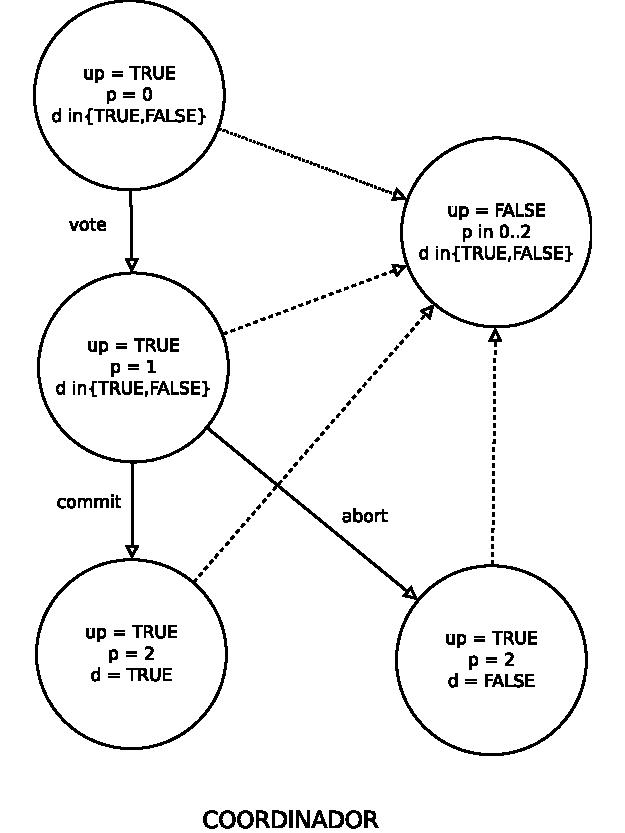
\includegraphics[scale=0.75]{Imagenes/2pcCoor.pdf}
  \caption{Diagrama de estados de una componente coordinador del protocolo de commit at\'omico de 2 fases}
  \label{2pcc}
\end{figure}
~\\
\begin{figure}[htp]
  \centering
    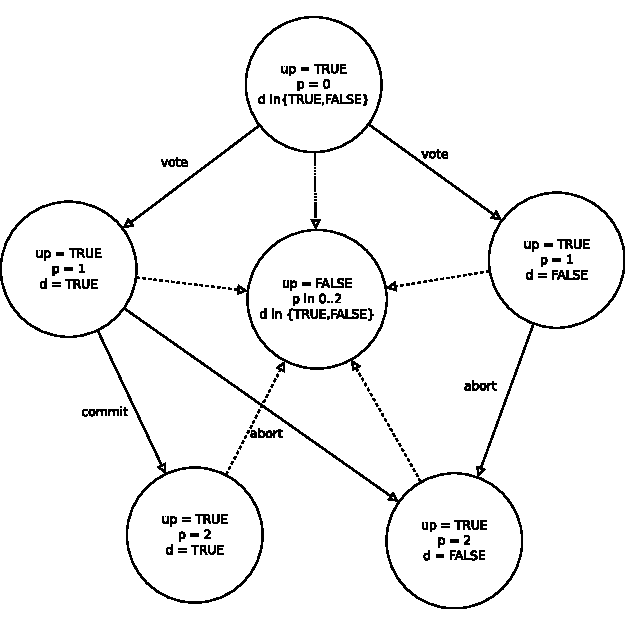
\includegraphics[scale=0.75]{Imagenes/2pcVoter.pdf}
  \caption{Diagrama de estados de una componente votante del protocolo de commit at\'omico de 2 fases}
  \label{2pcv}
\end{figure}
~\\

En nuestro caso de estudio no tomaremos en cuenta fallas en la comunicaci\'on entre los procesos, solo simularemos fallas de tipo STOP, simulando as\'i la ca\'ida en inactividad de alg\'un proceso interviniente. Quedar\'a abstra\'ida tambi\'en aquellas fallas que llevan a que los procesos voten por no hacer commit ya que no conciernen al protocolo. Miremos entonces el modelado de este protocolo en Falluto2.0, tomando el caso de 4 votantes y un coordinador. Comenzamos modelando la clase de proceso coordinador:\\

\noindent \line(1,0){400}
\begin{verbatim}
PROCTYPE Coordinator(v0, v1, v2, v3)

    VAR
        p   : 0..2
        d   : bool
        up  : bool
    
    FAULT 
        crash: => up' = FALSE is STOP

    INIT
        p = 0 & up = TRUE

    TRANS
        [vote]:    p = 0 => p' = 1, d' in { TRUE, FALSE };
        [commit]:  p = 1 &
                   v0.up & v0.d & v0.p = 1 &
                   v1.up & v1.d & v1.p = 1 &
                   v2.up & v2.d & v2.p = 1 &
                   v3.up & v3.d & v3.p = 1 
                   => p' = 2, d' = TRUE;
        [abort]:  p = 1 &
                  ((!v0.up | (v0.p >= 1 & !v0.d)) |
                   (!v1.up | (v1.p >= 1 & !v1.d)) |
                   (!v2.up | (v2.p >= 1 & !v2.d)) |
                   (!v3.up | (v3.p >= 1 & !v3.d)) |
                   !d)
                  => p' = 2, d' = FALSE;
ENDPROCTYPE
\end{verbatim}
\line(1,0){400}
~\\\\

Como vemos el modelado surge de manera directa a partir de la especificaci\'on. Miremos sin embargo con detenci\'on la secci\'on \textbf{FAULT} del modelado del proceso coordinador. En ella encontramos la especificaci\'on de una \'unica falla, representando la detenci\'on del proceso. Esta falla es por ende de tipo \textit{STOP}, y como vimos es de car\'acter permanente, es decir que una vez que ocurre, el proceso instanciado quedar\'a infinitamente inhabilitado para realizar cualquier transici\'on buena. Dado que es de nuestro inter\'es que los dem\'as procesos puedan enterarse de la ocurrencia de la falla, o mas bien de la detenci\'on del proceso coordinador, hemos agregado a la falla de detenci\'on la postcondici\'on \textit{up' = FALSE}. Veremos mas adelante como los dem\'as procesos pueden acceder a esta variable, en funci\'on de variable de contexto, y de esta manera enterarse de la situaci\'on del coordinador. Vale la pena tambi\'en revisar los par\'ametros de contexto de esta declaraci\'on. Como vemos posee 4 variables de contexto: \textit{--~v0, v1, v2, v3~--}. Cada una de estas ser\'a una referencia a cada votante en el sistema, y ser\'an especificados en la instanciaci\'on al realizar el pasaje de par\'ametros. De este modo el proceso coordinador podr\'a en cualquier momento acceder a las variables de estado de los votantes en condici\'on de solo lectura.\\

Continuando con el modelado, miremos ahora los procesos votantes:\\

\noindent \line(1,0){400}
\begin{verbatim}
PROCTYPE RegularVoter(coo, v0, v1, v2)
    
    VAR
        p:  0..2
        d:  bool
        up: bool

    FAULT
        crash: => up' = FALSE is STOP
    
    INIT
        p = 0 & up = TRUE

    TRANS
        [vote]: p = 0 & coo.up & coo.p = 1
                => 
                d' in {TRUE, FALSE}, p' = 1;
        [abort]: p = 0 & !coo.up => p' = 2, d' = FALSE;
        [commit]: p < 2 & coo.p = 2 => p' = 2, d' = coo.d;
        [commit]: p < 2 & v0.p = 2 => p' = 2, d' = v0.d;
        [commit]: p < 2 & v1.p = 2 => p' = 2, d' = v1.d;
        [commit]: p < 2 & v2.p = 2 => p' = 2, d' = v2.d;

ENDPROCTYPE
\end{verbatim}
\line(1,0){400}
~\\\\


Nuevamente el modelado se extrae de manera directa de la especificaci\'on del algoritmo. Vemos como cada proceso tiene acceso en forma de solo lectura a cada uno de los dem\'as procesos en el sistema, incluyendo al coordinador (\textit{coo}). La falla declarada es id\'entica a la declarada en el modelado del coordinador. Por \'ultimo la acci\'on \textit{commit} fue separada para cada caso en que se detecta la toma de decisi\'on de un proceso diferente. Si bien comparten el nombre, solo una de ellas ser\'a elegida para realizar la transici\'on.\\

Miremos ahora como organizar los procesos en la etapa de instanciaci\'on de manera que cada uno pueda ver el estado de los dem\'as. Para instanciar los procesos usaremos el siguiente c\'odigo:\\

\noindent \line(1,0){400}
\begin{verbatim}
INSTANCE coord = Coordinator(voter0, voter1, voter2, voter3)
INSTANCE voter0 = RegularVoter(coord, voter1, voter2, voter3)
INSTANCE voter1 = RegularVoter(coord, voter0, voter2, voter3)
INSTANCE voter2 = RegularVoter(coord, voter0, voter1, voter3)
INSTANCE voter3 = RegularVoter(coord, voter0, voter2, voter1)
\end{verbatim}
\noindent \line(1,0){400}
~\\\\

Como vemos, hemos instanciado un proceso coordinador y cuatro procesos votantes. Hemos asignado los nombres de instanciaci\'on de cada proceso como par\'ametros de los dem\'as procesos en el orden correspondiente de manera que tenga sentido el modelado de los proctypes. Esto queda claro en el caso de los procesos votantes, donde el \'indice del par\'ametro para el proceso coordinador en la instanciaci\'on coincide con el \'indice de la variable de contexto \textit{coo} en el proctype \textit{RegularVoter}.\\

Una vez modelado el sistema, es necesario especificar las propiedades deseadas sobre el mismo, para su posterior verificaci\'on con la herramienta. Vimos en la especificaci\'on del algoritmo que estamos trabajando, que buscamos que el mismo cumpla con tres propiedades especificas. Las recordamos a continuaci\'on y miramos el c\'odigo usado para especificarlas en Falluto2.0:
\begin{enumerate}
\item \textbf{Si no ocurren errores y todos los procesos votan por \textbf{SI}, entonces todos los procesos llegan a la decisi\'on de commit.}\\ Esta propiedad supone que no ocurren errores y en ese contexto busca probar que si todos los procesos votaron por hacer commit entonces todos llegan a la decisi\'on de hacer commit. Podemos aprovechar entonces la metapropiedad \textit{NORMAL\_BEHAIVIOUR} para este caso, y la especificaci\'on en Falluto2.0 tomar\'a entonces la siguiente forma:\\
\noindent \line(1,0){350}
\begin{verbatim}
NORMAL_BEHAIVIOUR -> G ( (coord.p = 1 & coord.d & 
                          voter0.p = 1 & voter0.d & 
                          voter1.p = 1 & voter1.d & 
                          voter2.p = 1 & voter2.d & 
                          voter3.p = 1 & voter3.d) 
                          -> 
                          F (coord.p = 2 & coord.d & 
                             voter0.p = 2 & voter0.d & 
                             voter1.p = 2 & voter1.d & 
                             voter2.p = 2 & voter2.d & 
                             voter3.p = 2 & voter3.d)
                       )
\end{verbatim}
\noindent \line(1,0){350}
~\\\\

\item \textbf{Un proceso llega a la decisi\'on de commit solo si todos los procesos votaron \textbf{SI}.}\\ Notemos que dado un proceso \textit{j} denotamos el estado en el que este proceso llega a la desici\'on de commit con el estado dado por las condiciones \textit{j.p = 2} y \textit{j.d = TRUE}. As\'i tambi\'en, sabemos que si un proceso \textit{j} se encuentra en una fase que no sea \textit{0}, y su variable \textit{d} tiene el valor booleano \textit{TRUE} entonces se puede decir que el proceso a votado a favor del commit. De este modo la especificaci\'on de esta propiedad en Falluto2.0 toma la forma:\\
\noindent \line(1,0){350}
\begin{verbatim}
LTLSPEC G ( ((coord.p = 2 & coord.d) |
             (voter0.p = 2 & voter0.d) |            
             (voter1.p = 2 & voter1.d) |
             (voter2.p = 2 & voter2.d) |
             (voter3.p = 2 & voter3.d) |
            )
            -> 
            (voter0.p != 0 & voter0.d & 
             voter1.p != 0 & voter1.d & 
             voter2.p != 0 & voter2.d & 
             voter3.p != 0 & voter3.d
            )
          ) 
\end{verbatim}
\noindent \line(1,0){350}
~\\\\

\item \textbf{Todos los procesos que llegan a una decisi\'on, llegan a la misma.}\\ Miremos esta propiedad en particular para los procesos \textit{voter1} y \textit{voter3}, ya que los dem\'as casos son semejantes. Supongamos que cada uno ha llegado a una decisi\'on y veamos que sea la misma. La siguiente sintaxis especifica esta propiedad como una propiedad en CTL:\\
\noindent \line(1,0){350}
\begin{verbatim}
CTLSPEC AG ( (voter1.p = 2 & voter3.p = 2) 
             -> 
             (voter1.d = voter3.d)
           )
\end{verbatim}
\noindent \line(1,0){350}
~\\\\

\end{enumerate}

Si verificamos con Falluto2.0 el modelo que hemos ido definiendo, junto con las propiedades especificadas, notaremos que en efecto el modelo las cumple. Falluto2.0 expondr\'a, por cada propiedad presentada, una linea asegurando las satisfactibilidad de la misma en el modelo.



\section{Protocolo de ventana deslizante\\GO-BACK-N}

Los \textit{protocolos de ventana deslizante} pertenecen al conjunto de protocolos de transmisi\'on de datos con control de error (ARQ), com\'unmente presentes en los algoritmos de capas de enlace de datos. Estos protocolos se caracterizan por el uso de \textit{n\'umeros de secuencia} en sus tramas, y el env\'io de \textit{mensajes de confirmaci\'on de recepci\'on}.\\

En los \textit{protocolos de ventana deslizante}, en cualquier instante, el emisor mantiene un grupo de de n\'umeros de secuencia que corresponde a las tramas que tiene permitido enviar. Se dice que estas tramas caen dentro de la ventana emisora. De manera semejante, el receptor mantiene una ventana receptora correspondiente al grupo de tramas que tiene permitido aceptar. Los n\'umeros de secuencia en la ventana del emisor representan tramas enviadas, o que pueden ser enviadas, pero cuya recepci\'on a\'un no ha sido confirmada. Una vez que se recibe la confirmaci\'on de alguna trama en la ventana, se hace lugar en la misma para el env\'io de una nueva trama. La ventana receptora corresponde, como ya dijimos, a las tramas que puede aceptar. Toda trama que caiga fuera de la ventana se descarta sin m\'as. Cuando se recibe una trama cuyo n\'umero de secuencia se corresponde con el l\'imite inferior de la ventana, esta trama se acepta, se genera un mensaje de confirmaci\'on de recepci\'on, y la ventana avanza para permitir la recepci\'on de una nueva trama de ser necesario. De este evento surge el nombre de este grupo de protocolos. Las ventanas de recepci\'on conservan su tama\~no inicial siempre\cite[tanembaum].\\

El protocolo \textbf{GO-BACK-N} es un caso espec\'ifico de protocolos de ventana deslizante, en donde el \textit{tama\~no de la ventana de recepci\'on es 1}. Este protocolo se caracteriza por la retransmisi\'on de tramas en tiempos en que el emisor en otro caso quedar\'ia ocioso. En particular, si el emisor ha enviado todas las tramas de su ventana y no ha recibido confirmaci\'on de recepci\'on para ninguna de ellas, entonces proceder\'a a retransmitir todas las tramas desde la \'ultima con confirmaci\'on de recepci\'on. Esta caracter\'istica representa un uso mas eficiente de la conexi\'on con respecto a los protocolos de detenci\'on y espera, ya que por un lado el emisor no debe esperar confirmaci\'on de recepci\'on para seguir enviando tramas dentro de su ventana, y por otro lado en el caso de p\'erdidas de paquetes, este se anticipa al reenv\'io de los mismos. Este tipo de protocolos es muy \'util en situaciones en las que retardo en los canales de transmisi\'on es muy grande, ya que en el caso de no retransmitir los tiempos de ocio del emisor ser\'ian muy elevados.\\

Con la intenci\'on de modelar el algoritmo que especifica este protocolo, dividiremos el mismo en cuatro partes:
\begin{enumerate}
\item \textbf{Env\'io de trama de secuencia}
\item \textbf{Recepci\'on de trama de secuencia}
\item \textbf{Env\'io de tramas de confirmaci\'on de recepci\'on}
\item \textbf{Recepci\'on de tramas de confirmaci\'on de recepci\'on}
\end{enumerate}
~\\

El emisor utilizar\'a entonces los algoritmos (1) y (4) mientras que el receptor los algoritmos (2) y (3). A continuaci\'on describiremos cada uno de estos algoritmos y mostraremos como modelarlos con Falluto2.0. Nuestra intenci\'on ser\'a modelar un nodo emisor y uno receptor, comunicados por canales no confiables, es decir por canales sujetos a la perdida de mensajes. Buscaremos demostrar con nuestra herramienta que este protocolo es tolerante a un numero de ocurrencia finito de estas fallas sobre los canales, en cuanto a que eventualmente todos las tramas podr\'an ser entregadas al receptor.\\\\

\begin{center}
\textbf{\large Los algoritmos (1) y (4), y el modelado del emisor.}
\end{center}

El siguiente pseudoc\'odigo representa el algoritmo de env\'io de trama de secuencia:\\

\noindent \line(1,0){400}
\begin{verbatim}
if( buffer de envio vacio )

    if( estoy restransmitiendo )
        continuo con la retransmision;
            
    else if( tengo tramas y la ventana no esta llena )
        envio trama nueva;

    else 
        inicio retransmision;

else
        
    continuar   		
        
\end{verbatim}
\noindent \line(1,0){400}\\\\

mientras que este otro representa al de recepci\'on de confirmaci\'on de recepci\'on:\\

\noindent \line(1,0){400}
\begin{verbatim}
if( la confirmacion cae dentro de la ventana de emision)
    
    deslizo la ventana;

    if( estoy retransmitiendo)

        dejo de retransmitir;

else

    descarto la confirmacion;
\end{verbatim}
\noindent \line(1,0){400}\\\\

Como vemos, iniciaremos la retransmisi\'on de tramas solo cuando hayamos enviado todos los paquetes dentro de nuestra ventana. A su vez detendremos la retransmisi\'on al recibir tramas de confirmaci\'on v\'alidas, ya que en ese caso se avanza la ventana y nuevas tramas se hacen disponibles para la retransmisi\'on. Notemos adem\'as que suponemos que siempre tenemos paquetes nuevos para insertar en nuestras tramas y enviarlos.\\

El modelado del emisor en Falluto2.0 presenta entonces el siguiente aspecto:\\

\noindent \line(1,0){400}
\begin{verbatim}
-- DEFINICIONES
DEFINE WZ := 2          -- Window size.
DEFINE MSEQ := 2        -- Max sequence number.
DEFINE MSP1 := MSEQ + 1 -- Max sequence number + 1.

PROCTYPE sender( ACK; send, read)

VAR
    DTX:  0..2 -- Data in output buffer
    NS:   0..2 -- Next sequence number
    LA:   0..2 -- Last Ack
    RT:   0..2 -- Retransmition index
    SENT: bool -- Output buffer empty?

INIT
    NS = 0 & LA = 0 & DTX = 0 & SENT & RT =  0

TRANS

    -- CONTINUAR CON LA RETRANSMISION SI SE HA EMPEZADO
    [contRetr]: RT != NS & SENT 
                => 
                DTX' = RT, RT' = (RT+1)%MSP1, SENT' = FALSE;

    -- NUEVO FRAME 
    [new]:  RT = NS & SENT & 
            ((NS >= LA & NS-LA < WZ)|(NS < LA & MSP1-LA+NS < WZ))
            => 
            SENT' = FALSE, NS' = (NS+1)%MSP1, 
            RT' = (RT+1)%MSP1, DTX' = NS;

    -- COMENZAR RETRANSMISION SI LA VENTANA ESTA LLENA
    [startRetr]: 
        ((NS>=LA & NS-LA >= WZ)|(NS<LA & MSP1-LA+NS >= WZ)) & 
        SENT & RT = NS 
        => 
        SENT' = FALSE, DTX' = LA, RT' = LA;


    -- LEER ACK INVALIDO Y DESCARTARLO
    [read]: !(NS > LA & (ACK > LA | ACK <= NS)) & 
            !(NS <= LA & ACK > LA & ACK <= NS);

    -- LEER ACK VALIDO Y ACEPTARLO
    [read]: (NS>LA & (ACK>LA | ACK<=NS)) |
            (NS <= LA & ACK > LA & ACK <= NS) 
            => 
            LA' = ACK, RT' = NS;


    -- ENVIAR EL MENSAJE POR EL CANAL DE COMUNICACION
    [send]: !SENT => SENT' = TRUE;

ENDPROCTYPE
\end{verbatim}
\noindent \line(1,0){400}\\

Hemos simulado un emisor sin fallas, el cual memoriza el valor de la \'ultima confirmaci\'on de recepci\'on, el n\'umero de secuencia del pr\'oximo paquete a ser enviado y el \'indice de retransmisi\'on. De esta manera la ventana de transmisi\'on queda definida entre los \'indices dados por \textit{LA} y \textit{NS}, y en caso de retransmisi\'on, el \'indide \textit{RT} recorre esta ventana simulando enviar las tramas correspondientes.\\

La secci\'on \textit{TRANS} del emisor, se ha definido tomando en cuenta el sentido de las construcciones \textit{IF-ELSEIF-ELSE}. Por lo tanto la guarda de cada transici\'on definida se conforma, en parte, por la negaci\'on de las guardas de las transiciones correspondientes a los casos anteriores dentro de la construcci\'on \textit{IF-ELSEIF-ELSE}. Las tres primeras transiciones se corresponden al algoritmo para env\'io de tramas de secuencia, mientras que las transiciones 4 y 5 pertenecen al de recepci\'on de tramas de confirmaci\'on de recepci\'on.\\


\begin{center}
\textbf{\large Los algoritmos (2) y (3), y el modelado del receptor.}
\end{center}

Miremos ahora el pseudoc\'odigo correspondiente a los algoritmos de recepci\'on de tramas de secuencia y env\'io de confirmaci\'on de recepci\'on. Estos algoritmos ser\'an inclu\'idos en el modelado del receptor.\\

El siguiente pseudoc\'odigo describe el algoritmo de recepci\'on de tramas de secuencia:\\

\noindent \line(1,0){400}\\

\begin{verbatim}
if( es la trama que esperaba )

    aceptar trama y correr ventana;
    generar confirmacion de recepcion;
    
else

    descartar trama;
    re-generar confirmacion de recepcion;
\end{verbatim}

\noindent \line(1,0){400}\\

El algoritmo para env\'io de tramas de confirmaci\'on de recepci\'on es muy simple ya que solo consta de enviar el n\'umero de secuencia que se espera recibir en la pr\'oxima trama. Ya que en el caso del protocolo GO-BACK-N, la ventana de recepci\'on posee tama\~no 1, el algoritmo consistir\'a en enviar el n\'umero de secuencia correspondiente a la nueva ventana obtenida luego de la recepci\'on de una trama v\'alida.\\

Miremos a continuaci\'on nuestro modelado del receptor en el lenguaje de Falluto2.0:\\

\noindent \line(1,0){400}\\

\begin{verbatim}
PROCTYPE receiver( NF; send, read)

VAR
        NR:0..2 -- Next request number
        NA:bool -- Need to send ack

INIT
        NR = 0 & NA = FALSE

TRANS

        -- DESCARTAR TRAMA INVALIDA
        [read]: NF != NR => NA' = TRUE;

        -- RECIBIR TRAMA VALIDA
        [read]: NF = NR => NR' = (NR+1)%(MSP1), NA' = TRUE;

        -- ENVIAR ACK DE SER NECESARIO
        [send]: NA => NA' = FALSE;

ENDPROCTYPE
\end{verbatim}

\noindent \line(1,0){400}\\

Hemos modelado entonces un receptor sin fallas, el cual mantiene memoria el n\'umero de secuencia de la pr\'oxima trama que se espera recibir. En su secci\'on \textit{TRANS} podemos distinguir el modelado de los algoritmos (2) y (3). Las dos primeras transiciones forman parte de la recepci\'on de tramas de secuencia, mientras que la \'ultima transici\'on describe el env\'io de la una trama de confirmaci\'on de recepci\'on.\\

A continuaci\'on modelaremos los canales de comunicaci\'on entre el emisor y el receptor. Estos canales estar\'an sujetos a fallas, en particular a fallas que implican la perdida de los mensajes que intentan atravesarlos. A continuaci\'on encontramos el modelo de los canales en el lenguaje de Falluto2.0:

\noindent \line(1,0){400}

\begin{verbatim}
PROCTYPE channel( IN; send, read )

VAR
    buff:  array 0..2 of 0..1 -- fisical channel
    data:  0..2               -- output data
    empty: bool               -- output buffer empty?

FAULT
    loose0: buff[0] > 0 => buff[0]' = buff[0]-1 is TRANSIENT
    loose1: buff[1] > 0 => buff[1]' = buff[1]-1 is TRANSIENT
    loose2: buff[2] > 0 => buff[2]' = buff[2]-1 is TRANSIENT
    
INIT
    buff[0] = 0 & buff[1] = 0 & buff[2] = 0 & empty & data = 0

TRANS
    -- ENVIAR UNA TRAMA POR EL CANAL
    [send]: IN = 0 & buff[0] < MAXCOP => buff[0]' = buff[0]+1;
    [send]: IN = 1 & buff[1] < MAXCOP => buff[1]' = buff[1]+1;
    [send]: IN = 2 & buff[2] < MAXCOP => buff[2]' = buff[2]+1;

    -- UNA TRAMA LLEGA AL FINAL DEL CANAL
    [arrive]: empty & buff[0] > 0 
              => 
              data' = 0, empty' = FALSE, buff[0]' = buff[0]-1;
    [arrive]: empty & buff[1] > 0 
              => 
              data' = 1, empty' = FALSE, buff[1]' = buff[1]-1;
    [arrive]: empty & buff[2] > 0 
              => 
              data' = 2, empty' = FALSE, buff[2]' = buff[2]-1;

    -- LA TRAMA ES LEIDA POR EL RECEPTOR DEL CANAL
    [read]: !empty => empty' = TRUE;

ENDPROCTYPE

\end{verbatim}

\noindent \line(1,0){400}\\

En el modelado de los canales tenemos que la variable \textit{buff} en la posici\'on $i$ define la cantidad de mensajes con n\'umero de secuencia $i$ que presentes en el canal. Por otro lado la variable \textit{data} representa la trama que ha arribado a destino para ser le\'ida por el receptor. A su vez la variable \textit{empty} indica si el receptor ya ha le\'ido el dato que le lleg\'o o no. Podemos distinguir tres tipos de transiciones en este modelado: las de nombre \textit{send} representan la introducci\'on de un mensaje en el canal por parte del emisor del mismo; las de nombre \textit{arrive} representan el arribo de la trama al extremo del canal donde ser\'a le\'ido; y por \'ultimo la transici\'on de nombre \textit{read} representa la lectura de la trama por parte del receptor del canal.\\

Hemos modelado las fallas de manera muy sencilla gracias a la lenguaje declarativo que otorga nuestra herramienta para la inyecci\'on de las mismas. De esta manera en una simple linea de la forma: $$ loosei:~buff[i]~>~0~=>~buff[i]'~=~buff[i]-1~is~TRANSIENT $$ hemos definido la falla que representa la perdida de una trama de n\'umero de secuencia $i$. Notemos que el nombre de la falla es $loosei$, mientras que la condici\'on de habilitaci\'on representa la necesidad de que en efecto exista un mensaje en el canal para que el mismo se pierda $( buff[i] > 0 )$. Por otro lado declaramos el efecto de perdida reduciendo la cantidad de tramas de n\'umero de secuencia $i$ en el canal usando la post-condici\'on $buff[i]' = buff[i]-1$, y declaramos que la falla es de tipo $TRANSIENT$ indicando que la misma puede ocurrir reiteradamente en cualquier momento durante la ejecuci\'on siempre que se cumpla su condici\'on de habilitaci\'on.\\

Por \'ultimo veamos como modelar el sincronizado de los canales con el emisor y el receptor mediante el pasaje de nombres de acci\'on comunes en la etapa de instanciaci\'on. Instanciamos entonces un emisor, un receptor, y dos canales, uno desde el emisor al receptor y otro en direcci\'on contraria. Hacemos esto de la siguiente manera:\\

\noindent \line(1,0){400}
\begin{verbatim}
INSTANCE emisor   = sender   (buffRE.data , send1, read1)
INSTANCE receptor = receiver (buffER.data , send2, read2)
INSTANCE buffER   = channel  (emisor.DTX  , send1, read2)
INSTANCE buffRE   = channel  (receptor.NR , send2, read1)
\end{verbatim}
\noindent \line(1,0){400}\\

De esta manera hemos logrado que el emisor pueda leer los datos que llegan a trav\'es del canal \textit{buffER} al pasar como par\'ametro la variable \textit{buffRE.data}. De manera similar el receptor recibe los datos desde el canal \textit{bufferRE} a trav\'es de la variable \textit{bufferRE.data} pasada como par\'ametro. A su vez cada canal puede leer los datos de salida de su emisor correspondiente a partir del pasaje de los par\'ametros \textit{emisor.DTX} y \textit{receptor.NR}. La sincronizaci\'on de las acciones \textit{read} y \textit{send} tanto del emisor y el receptor con sus canales correspondientes se logra pasando como par\'ametro nombres equivalentes para las acciones.\\

Nos interesa probar ciertas propiedades sobre este modelo. Una de ellas expresa que cierto n\'umero de secuencia llegue siempre a menudo al receptor. Usemos en particular el n\'umero m\'aximo de secuencia y revisemos si se cumple que el receptor lo recibe siempre a menudo. De acuerdo al modelado que hemos realizado podemos identificar la llegada de una trama con n\'umero de secuencia m\'aximo como la ocurrencia de una lectura del canal por parte del emisor, en momento en que la variable \textit{data} del canal correspondiente contiene el valor \textit{MSEQ}. Queremos entonces describir en lenguaje de Falluto una propiedad que exprese que \textit{para toda ejecuci\'on suceda que siempre a menudo \textbf{canalER.data = MSEQ $\&$ receptor lee el canal }}. Encontramos que la sintaxis de Falluto2.0 ofrece una manera muy sencilla de describir la acci\'on en la cual el receptor lee el canal, usando la construcci\'on \textit{just()}. Obtenemos entonces usando el lenguaje de Falluto2.0. la siguiente formula LTL para expresar la propiedad que hemos sugerido: \\

\noindent \textbf{Propiedad(1):}\\ \textit{LTLSPEC G F (canalER.data = MSEQ \& just(read2))}

Podemos verificar la veracidad de esta propiedad bajo escenarios en los que las fallas no ocurren usando la meta-propiedad \textit{NORMAL\_BEHAIVIOUR}, y bajo escenarios en los que la ocurrencia de fallas es de car\'acter finito usando la meta-propiedad \textit{FINITELY\_MANY\_FAULTS}. Las propiedades resultantes del uso de estas meta-propiedades tienen la siguiente forma:\\

\noindent \textbf{Propiedad(2):}\\ \textit{NORMAL\_BEHAIVIOUR $\rightarrow$ G~F~(canalER.data = MSEQ~\&~just(read2))}\\

\noindent \textbf{Propiedad(3):}\\ \textit{FINITELY\_MANY\_FAULTS $\rightarrow$ ~G~F~(canalER.data = MSEQ~\&~just(read2))}\\


Como resultado de la verificaci\'on realizada por Falluto2.0 obtendremos que solo las propiedades (1) y (3) se cumplen, mientras que un contraejemplo sera presentado para refutar la propiedad(2). 

%\section{Ej\'ercitos bizantinos ?}
%\section{Fil\'osofos comensales ?}
%\section{Falla bizantina ?}
%\section{Elecci\'on de lider ?}
%\section{Protocolos lamport}
%\section{Feedback de contacto de Naza}
%\section{Red satelital ultra secreta?}


%%%%%%%%%%%%%%%%%%%%%%%%%%%%%%%%%%%%%%%%%%%%%%%%%%%%%%%%%%%%%%%%%%%%%%%%%%%%%%%%%%%%%%%%%%%%%%%%%%%%%%%%%%%%%%%%%%%%%%%%%%%%%%%%%%%%%%%%%%%%%%%%%%%%%%%%%%%%%%%%%%

\chapter{Conclusi\'on}



\appendix
\appendixpage
\noappendicestocpagenum
\addappheadtotoc

\chapter{Manual de Falluto2.0}
Mostraremos en este ap\'endice los pasos a seguir para preparar el entorno operativo para Falluto2.0. Detallaremos adem\'as como utilizarlo para la verificaci\'on de nuestros sistemas tolerantes a fallas, describiendo cada una de las opciones y utilidades que la herramienta ofrece.

\section{Instalaci\'on de Falluto2.0}
Previo a poder utilizar Falluto2.0 en nuestra PC debemos preparar el entorno en nuestro sistema Linux. Para ello precisamos poseer instalado tanto NuSMV versi\'on 2.5.3 o superior, como as\'i tambi\'en Python versi\'on 2.6.5 o superior. Tanto NuSMV como Python deben ser accesible mediante la ruta de busqueda para ejecuci\'on 'PATH'.

\section{Opciones y utilizaci\'on de la herramienta}
El primer paso para la verificaci\'on del sistema es poseer un archivo (por convenci\'on terminado en .fll) en el cual se encuentre la descripci\'on del sistema junto con las opciones de verificaci\'on y las propiedades a verificar (Ver el manual de usuario de Falluto2.0 para mayores indicaciones). Dentro de la carpeta de instalaci\'on de Falluto2.0 encontramos el script ejecutable del programa llamado \textit{Falluto2.0.py}. Ejecutamos este script con las siguientes opciones para realizar la verificaci\'on:\\


\noindent usage: Falluto2.0 [-h] [--version] [-s path] [-co] filename\\


\begin{tabular}{ll}
\textbf{argumentos posicionales:}\\\\
filename & Ruta del archivo de input donde se encuentra \\
         & la descripci\'on del sistema.\\
\textbf{argumentos opcionales:} & \\\\
-h, --help          & muestra este mensaje de ayuda.\\
--version           & muestra la versi\'on de este programa y sale.\\
-s path, --s path, -save path & guardar la versi\'on compilada a NuSMV de este \\
                              & sistema en el archivo dado por la ruta 'path'.\\
-co 		        & output con color.\\
\end{tabular}



%%%%%%%%%%%%%%%%%%%%%%%%%%%%%%%%%%%%%%%%%%%%%%%%%%%%%%%%%%%%%%%%%%%%%%%%%%%%%%%%%%%%%%%%%%%%%%%%%%%%%%%%%%%%%%%%%%%%%%%%%%%%%%%%%%%%%%%%%%%%%%%%%%%%%%%%%%%%%%%%%%


\chapter{Sint\'axis formal de Falluto}
\label{sintaxisFormal}

A continuaci\'on presentamos la sint\'axis formal de Falluto2.0 en t\'erminos de Parsing Expression Grammars (PEG) y Regular Expressions (RE). Estas producciones pasan por alto los espacios en blanco, tabulaciones y saltos de linea. Consideramos aqu\'i terminales a las letras en it\'alico, y a los s\'imbolos y puntuaciones entre comillas.

\section{Palabras reservadas de Falluto2.0}

Las siguientes palabras son de caracter reservado, son usadas para fines espec\'ificos en la especificaci\'on del sistema, y no pueden ser usadas como identificadores de variables o nombres.\\

%\begin{tabular}{>{\bfseries}l>{\itshape}l}
\begin{tabularx}{\textwidth}{>{\bfseries}l>{\itshape}X }

RESERVED $\longleftarrow$ & in / CHECK\_DEADLOCK / OPTIONS / ENDOPTIONS / SYSNAME / just / is / FAIRNESS / COMPASSION / U / V / S / T / xor / xnor / G / X / F / H / O / Z / Y / PROCTYPE / ENDPROCTYPE / INSTANCE / TRANS / INIT / VAR / FAULT / TRUE / FALSE / AG / AX / AF / EX / EF / EG / INST\_WEAK\_FAIR\_DISABLE / FAULT\_FAIR\_DISABLE / in / FINITELY\_MANY\_FAULT / FINITELY\_MANY\_FAULTS / LTLSPEC / CTLSPEC / DEFINE / FAIRNESS / COMPASSION/ NORMAL\_BAHAIVIOUR\\
\end{tabularx}
%\end{tabular}
~\\



\section{Algunas producciones simples}

Identificadores pueden contener '.' para indicar pertenencia a un proceso espec\'ifico ( por ejemplo instancia.variable ). Nombres en cambio no.\\

~\\\\
\begin{tabularx}{\textwidth}{>{\bfseries}llX}
IDENT & $\longleftarrow$ & ! RESERVED [a-zA-Z\_](``.''[a-zA-Z0-9\_]+)?\\\\
NAME & $\longleftarrow$ & ! RESERVED [a-zA-Z\_][a-zA-Z0..9\_]*\\\\
INT & $\longleftarrow$ & -? ( [0] / [1-9][0-9]* )\\\\
BOOL & $\longleftarrow$ & ``TRUE'' / ``FALSE''\\\\
EVENT & $\longleftarrow$ & ``just('' IDENT ``)''\\\\
NEXTREF & $\longleftarrow$ & IDENT `` ' ''\\\\
RANGE & $\longleftarrow$ & INT ``..'' INT\\\\
BOOLEAN & $\longleftarrow$ & ``bool''\\\\
SET & $\longleftarrow$ & ``\{'' (IDENT / INT / BOOL) (``,'' (IDENT / INT / BOOL))* ``\}''\\\\
INCLUSION & $\longleftarrow$ & IDENT ``in'' (SET / RANGE)\\
\end{tabularx}
~\\\\

\section{Expresiones}
Las expresiones describen formulas booleanas o enteras. A continuaci\'on encontramos su sintaxis:

\begin{tabularx}{\textwidth}{>{\bfseries}llX }

%\noindent \begin{longtable}{>{\bfseries}ll>{\itshape}l}
EXPRESION & $\longleftarrow$ & PROP\\\\
PROP & $\longleftarrow$ & CONJ ( ('$->$' / '$<->$') PROP ) ?\\\\
CONJ & $\longleftarrow$ & COMP ( ('$|$' / '$\&$') CONJ ) ?\\\\
COMP & $\longleftarrow$ & PROD ( ('$<=$' / '$>=$' / '$\>>$' / '$\<<$' / '$!=$' / '$=$') CONJ ) ?\\\\
PROD & $\longleftarrow$ & SUM ( ('$*$' / '$\div$' / '$\%$' ) PROD ) ?\\\\
SUM & $\longleftarrow$ & VALUE ( ('$+$' / '$-$' ) SUM ) ?\\\\
VALUE & $\longleftarrow$  & ( '(' PROP ')' / INCLUSION / NEXTREF / IDENT / INT / BOOL / EVENT / ! VALUE / - VALUE ) \\\\
NEXTLIST & $\longleftarrow$  & NEXTASSIGN (',' NEXTASSIGN)*\\\\
NEXTASSIGN & $\longleftarrow$  & NEXTREF ( = EXPRESION / ``in'' ( SET / RANGE ) )\\
\end{tabularx}
~\\\\




\section{Proctypes}
Un sistema falluto se modela con un encabezado de opciones de configuraci\'on (opcional) y una serie de objetos pertenecientes a la lista -- PROCTYPE, DEFINE, INSTANCE, SPEC, CONTRAINT --:\\\\

%\noindent \begin{longtable}{>{\bfseries}lll}
%\begin{tabularx}{\textwidth}{>{\bfseries}llX }
\begin{longtable}{>{\bfseries}ll >{\raggedright}p{0.6\textwidth} }
SYSTEM & $\longleftarrow$ & OPTIONS ? ( DEFINE / PROCTYPE / INSTANCE / SPECIFICATION / CONTRAINT ) *\cr\cr
OPTIONS & $\longleftarrow$ & ``OPTIONS'' ( ``SYSNAME'' [a-z0-9A-Z$\_$.]* / ``CHECK\_DEADLOCK'' / ``FAULT\_FAIR\_DISABLE'' / ``INST\_WEAK\_FAIR\_DISABLE'' )* ``ENDOPTIONS''\cr\cr
DEFINE & $\longleftarrow$ & ``DEFINE'' IDENT $":="$  EXPRESION \cr\cr
PROCTYPE & $\longleftarrow$ & ``PROCTYPE'' IDENT ``('' CTXVARS ? SYNCACTS ? ``)'' PROCTYPEBODY ``ENDPROCTYPE''\cr\cr
CTXVARS & $\longleftarrow$ & IDENT (``,'' IDENT)*\cr\cr
SYNCACTS & $\longleftarrow$ & ';' IDENT (``,'' IDENT)*\cr\cr
PROCTYPEBODY & $\longleftarrow$ & VAR ? FAULT ? INIT ? TRANS ?\cr\cr
VAR & $\longleftarrow$ & ``VAR'' VARDECL*\cr\cr
VARDECL & $\longleftarrow$ & IDENT ``:'' (BOOLEAN / SET / RANGE)\cr\cr
FAULT & $\longleftarrow$ & ``FAULT'' FAULTDECL*\cr\cr
FAULTDECL & $\longleftarrow$ & NAME ``:'' (EXPRESION ? $``=>"$ NEXTEXPR ?) ? ``is'' (BYZ / STOP / TRANSIENT)\cr\cr
BYZ & $\longleftarrow$ & ``BYZ'' ``('' IDENT (``,'' IDENT)*, ``)''\cr\cr
TRANSIENT & $\longleftarrow$ & ``TRANSIENT''\cr\cr
STOP & $\longleftarrow$ & ``STOP'' ( ``('' IDENT, (``,'' IDENT)* ``)'' ) ?\cr\cr
INIT & $\longleftarrow$ & ``INIT'' EXPRESION ?\cr\cr
TRANS & $\longleftarrow$ & ``TRANS'' TRANSDECL*\cr\cr
TRANSDECL & $\longleftarrow$ & ``['' NAME? ``]'' ``:'' EXPRESION? ( $"=>"$ NEXTEXPR )?\cr
\end{longtable}
~\\\\



\section{Instanciaci\'on}
Para especificar que un proceso forma parte del sistema, debemos instanciar el mismo a partir de un proctype previamente definido. La sintaxis de instanciaci\'on de procesos es la que sigue:\\\\

\begin{longtable}{>{\bfseries}ll >{\raggedright}p{0.65\textwidth} }
INSTANCE & $\longleftarrow$ & ``INSTANCE'' NAME ``='' NAME ``('' INSTPARAMS ``)''\cr\cr
INSTPARAMS & $\longleftarrow$ & ( (IDENT / INT / BOOL) (``,'' (IDENT / INT / BOOL) )* ) ?
\end{longtable}
~\\\\



\section{Especificaci\'on de propiedades}
Usamos las siguientes reglas para especificar las propiedades a verificar sobre el sistema modelado. Encontramos que podemos definir propiedades tanto en l\'ogica LTL como en CTL. Podemos adem\'as hacer uso de mete-propiedades predefinidas para facilitar la verificaci\'on:\\

Para la elaboraci\'on de propiedades LTL y CTL, se ofrece la siguiente sintaxis:\\

\begin{longtable}{>{\bfseries}ll >{\raggedright}p{0.7\textwidth} }
SPEC 	  & $\longleftarrow$ & CTLSPEC / LTLSPEC / NORMALBEHAIVIOUR / FINMANYFAULTS / FINMANYFAULT\cr\cr
CTLSPEC   & $\longleftarrow$ &\textit{CTLSPEC} CTLEXP\cr\cr
CTLEXP 	  & $\longleftarrow$ & CTLVALUE CTLBINOP CTLEXP / (\textit{A} / \textit{E}) '[' CTLEXP \textit{U} CTLEXP ']' / CTLVALUE\cr\cr
CTLBINOP  & $\longleftarrow$ & '\&' / '$|$' / \textit{xor} / \textit{xnor} / $"->"$ / $"<->"$\cr\cr
CTLVALUE  & $\longleftarrow$ & CTLUNOP CTLEXP /'(' CTLEXP ')' / EXPRESION\cr\cr
CTLUNOP   & $\longleftarrow$ & \textit{$'!'$ / EG / EX / EF / AG / AX / AF}\cr\cr
LTLSPEC   & $\longleftarrow$ & \textit{LTLSPEC} LTLEXP\cr\cr
LTLEXP    & $\longleftarrow$ & LTLBOP / LTLUOP\cr\cr
LTLBOP    & $\longleftarrow$ & LTLUOP LTLBINOPS LTLEXP\cr\cr
LTLUOP    & $\longleftarrow$ & LTLUNOPS* LTLVAL\cr\cr
LTLVAL    & $\longleftarrow$ & EXPRESION / '(' LTLEXP ')'\cr\cr
LTLUNOPS  & $\longleftarrow$ & \textit{$!$ / G / X / F / H / O / Z / Y}\cr\cr
LTLBINOPS & $\longleftarrow$ & \textit{ U / V / S / T / xor / xnor / $'|'$ / $'\&'$ / $"<->"$ / $"->"$}\cr
\end{longtable}
~\\

A continuaci\'on encontramos las reglas sint\'acticas para el uso de las meta-propiedades de Falluto2.0:\\

\begin{longtable}{>{\bfseries}ll >{\raggedright}p{0.50\textwidth} }
NORMALBEHAIVIOUR & $\longleftarrow$ & \textit{NORMAL\_BEHAIVIOUR} $"->"$ (CTLEXP / LTLEXP)\cr\cr
FINMANYFAULTS & $\longleftarrow$ & \textit{FINITELY\_MANY\_FAULTS} $"->"$ LTLEXP\cr\cr
FINMANYFAULT & $\longleftarrow$ & \textit{FINITELY\_MANY\_FAULT} '(' IDENT (',' IDENT)* ')' $"->"$ LTLEXP\cr
\end{longtable}
~\\\\



\section{Restricciones y fairness}

Las siguientes son reglas sint\'acticas para la elaboraci\'on de restricciones de fairness sobre la verificaci\'on del sistema. Espec\'ificamente podemos definir dos tipos de restricciones de fairness: inconditional fairness (\textit{FAIRNESS}) y strong fairness (\textit{COMPASSION}).

\begin{longtable}{>{\bfseries}ll >{\raggedright}p{0.75\textwidth} }
CONTRAINT & $\longleftarrow$ & FAIRNESS / COMPASSION\cr\cr
FAIRNESS & $\longleftarrow$ & \textit{FAIRNESS} EXPRESION\cr\cr
COMPASSION & $\longleftarrow$ & \textit{COMPASSION} '(' EXPRESION ',' EXPRESION ')'\cr
\end{longtable}
~\\\\





%%%%%%%%%%%%%%%%%%%%%%%%%%%%%%%%%%%%%%%%%%%%%%%%%%%%%%%%%%%%%%%%%%%%%%%%%%%%%%%%%%%%%%%%%%%%%%%%%%%%%%%%%%%%%%%%%%%%%%%%%%%%%%%%%%%%%%%%%%%%%%%%%%%%%%%%%%%%%%%%%%


\chapter{Ejemplo paradigm\'atico de compilaci\'on.}





%%%%%%%%%%%%%%%%%%%%%%%%%%%%%%%%%%%%%%%%%%%%%%%%%%%%%%%%%%%%%%%%%%%%%%%%%%%%%%%%%%%%%%%%%%%%%%%%%%%%%%%%%%%%%%%%%%%%%%%%%%%%%%%%%%%%%%%%%%%%%%%%%%%%%%%%%%%%%%%%%%


\chapter{extra}
	- falencias de falluto??? 
	- fallas por omisi\'on de input.
	- recuperci\'on de fallas por parte del usuario.
%TODO Algo que le falta a Falluto 2.0 es la posibilidad de simular interactivamente sobre el sistema modelado para depurar el modelado mismo.



%%%%%%%%%%%%%%%%%%%%%%%%%%%%%%%%%%%%%%%%%%%%%%%%%%%%%%%%%%%%%%%%%%%%%%%%%%%%%%%%%%%%%%%%%%%%%%%%%%%%%%%%%%%%%%%%%%%%%%%%%%%%%%%%%%%%%%%%%%%%%%%%%%%%%%%%%%%%%%%%

\newpage % Bibliography goes in new page

\begin{thebibliography}{99}


\bibitem{faultInjection}
Clarke, J.A.; Pradhan, D.K.
\newblock {\em Fault injection: a method for validating computer-system dependability.}
\newblock {June.1995}


\bibitem{SteinerRushby} 
Steiner-etal:DSN04; Wilfried Steiner and John Rushby and Maria Sorea and Holger Pfeifer;
\newblock {\em Model Checking a Fault-Tolerant Startup Algorithm: From Design Exploration To Exhaustive Fault Simulation.}
\newblock The International Conference on Dependable Systems and Networks, IEEE Computer Society, Florence, Italy, june, 2004


\bibitem{RuysBrinksma}
Theo C. Ruys and Ed Brinksma.
\newblock {\em Model Checking: Verification or Debugging?} 
\newblock Faculty of Computer Science, University of Twente. P.O. Box 217, 7500 AE Enschede, The Netherlands.


\bibitem{NuSMV}
Roberto Cavada, Alessandro Cimatti, Charles Arthur Jochim, Gavin Keighren, Emanuele Olivetti, Marco Pistore, Marco Roveri and Andrei Tchaltsev.
\newblock {\em NuSMV 2.5 User Manual.}  
\newblock \texttt{http://nusmv.fbk.eu/NuSMV/userman/v25/nusmv.pdf}


\bibitem{Hames}
Edgardo~E.\ Hames.
\newblock \textsc{Falluto}: {U}n model checker para la verificaci\'on de
  sistemas tolerantes a falla.
\newblock Trabajo de grado, FaMAF, Universidad Nacional de C\'ordoba, 2009.


\bibitem{Bordenabe}
Nicol\'as Bordenabe.
\newblock \textsc{Offbeat}: {U}na extensi\'on de {PRISM} para el an\'alisis de
  sistemas temporizados tolerantes a fallas.
\newblock Trabajo de grado, FaMAF, Universidad Nacional de C\'ordoba, 2011.


\bibitem{Python} 
\newblock {\em Python.} 
\newblock \texttt{http://www.python.org/about/}


\bibitem{PEG}
Bryan Ford.
\newblock{ \em Parsing Expression Grammars: A Recognition-Based Syntactic Foundation.}
\newblock{ Massachusetts Institute of Technology; Cambridge, MA.}


\bibitem{Felix} 
FELIX C. GÄRTNER.
\newblock {\em Fundamentals of Fault-Tolerant Distributed Computing in Asynchronous Environments.}
\newblock Darmstadt University of Technology. ACM Computing Surveys, Vol. 31, No. 1, March 1999


\bibitem{FaultInject} 
Jeffrey A. Clarke Mitre Corporation, Dhiraj K. Pradhan.
\newblock {\em  Fault Injection. A Method For Validating Fomputer-System Dependability.}
\newblock  Texas A\&M University. June 1995


\bibitem{Cristian} 
Flavin Cristian.
\newblock {\em Understanding fault tolerant distributed systems.} 
\newblock COMMUNICATIONS OF THE ACM, February 1991, Vol.34, No.2


\bibitem{prinMC} 
Christel Baier and Joost-Pieter Katoen.
\newblock{\em Principles of model checking.} 
\newblock The MIT Press Cambridge, Massachusetts London, England.


\bibitem{Clarke} 
Edmund M. Clarke, Orna Grumberg, David E. Long.
\newblock {\em Model checking.}
\newblock NATO ASI DPD 1996: 305-349


\bibitem{Baier} 
Christel Baier and Joost-Pieter Katoen.
\newblock {\em Principles of Model Checking (Representation and Mind Series).}
\newblock The MIT Press, 2008.


\bibitem{Huth} 
Michael R A Huth, Mark D Ryan.
\newblock {\em Logic in Computer Science, Modeling and reasoning about systems.}
\newblock Cambridge University Press. 2000.


\bibitem{Cimatti} 
A. Cimatti, E. Clarke, F. Giunchiglia, M. Roveri. 
\newblock {\em \textsc{NuSMV}: a new Symbolic Model Verifier.}
\newblock In N. Halbwachs and D. Peled, editors. Proceeding of International Conference on Computer-Aided Verification (CAV'99). In Lecture Notes in Computer Science, number 1633, pages 495-499, Trento, Italy, July 1999. Springer.


\bibitem{Arora} 
A. Arora and M. G. Gouda. 
\newblock {\em Closure and convergence: A foundation of fault-tolerant computing.}
\newblock IEEE Trans. Software Eng., 19(11):1015–1027, 1993.


\bibitem{dCTL} 
P. F. Castro, C. Kilmurray, A. Acosta, N. Aguirre. 
\newblock {\em dCTL: A Branching Time Temporal Logic for Fault-Tolerant System Verification.}
\newblock SEFM 2011.


\bibitem{NuSMV2}
Cimatti, Alessandro; Clarke, Edmund M.; Giunchiglia, Enrico; Giunchiglia, Fausto; Pistore, Marco; Rovere, Marco; Sebastiani,
Roberto; and Tacchella, Armando.
\newblock {\em NuSMV 2: An OpenSource Tool for Symbolic Model Checking.}
\newblock Computer Science Department. Paper 430. 2002.
\newblock \texttt{http://repository.cmu.edu/compsci/430}


\end{thebibliography}

\end{document}
